\documentclass[twoside]{book}

% Packages required by doxygen
\usepackage{fixltx2e}
\usepackage{calc}
\usepackage{doxygen}
\usepackage[export]{adjustbox} % also loads graphicx
\usepackage{graphicx}
\usepackage[utf8]{inputenc}
\usepackage{makeidx}
\usepackage{multicol}
\usepackage{multirow}
\PassOptionsToPackage{warn}{textcomp}
\usepackage{textcomp}
\usepackage[nointegrals]{wasysym}
\usepackage[table]{xcolor}

% Font selection
\usepackage[T1]{fontenc}
\usepackage[scaled=.90]{helvet}
\usepackage{courier}
\usepackage{amssymb}
\usepackage{sectsty}
\renewcommand{\familydefault}{\sfdefault}
\allsectionsfont{%
  \fontseries{bc}\selectfont%
  \color{darkgray}%
}
\renewcommand{\DoxyLabelFont}{%
  \fontseries{bc}\selectfont%
  \color{darkgray}%
}
\newcommand{\+}{\discretionary{\mbox{\scriptsize$\hookleftarrow$}}{}{}}

% Page & text layout
\usepackage{geometry}
\geometry{%
  a4paper,%
  top=2.5cm,%
  bottom=2.5cm,%
  left=2.5cm,%
  right=2.5cm%
}
\tolerance=750
\hfuzz=15pt
\hbadness=750
\setlength{\emergencystretch}{15pt}
\setlength{\parindent}{0cm}
\setlength{\parskip}{3ex plus 2ex minus 2ex}
\makeatletter
\renewcommand{\paragraph}{%
  \@startsection{paragraph}{4}{0ex}{-1.0ex}{1.0ex}{%
    \normalfont\normalsize\bfseries\SS@parafont%
  }%
}
\renewcommand{\subparagraph}{%
  \@startsection{subparagraph}{5}{0ex}{-1.0ex}{1.0ex}{%
    \normalfont\normalsize\bfseries\SS@subparafont%
  }%
}
\makeatother

% Headers & footers
\usepackage{fancyhdr}
\pagestyle{fancyplain}
\fancyhead[LE]{\fancyplain{}{\bfseries\thepage}}
\fancyhead[CE]{\fancyplain{}{}}
\fancyhead[RE]{\fancyplain{}{\bfseries\leftmark}}
\fancyhead[LO]{\fancyplain{}{\bfseries\rightmark}}
\fancyhead[CO]{\fancyplain{}{}}
\fancyhead[RO]{\fancyplain{}{\bfseries\thepage}}
\fancyfoot[LE]{\fancyplain{}{}}
\fancyfoot[CE]{\fancyplain{}{}}
\fancyfoot[RE]{\fancyplain{}{\bfseries\scriptsize Generated by Doxygen }}
\fancyfoot[LO]{\fancyplain{}{\bfseries\scriptsize Generated by Doxygen }}
\fancyfoot[CO]{\fancyplain{}{}}
\fancyfoot[RO]{\fancyplain{}{}}
\renewcommand{\footrulewidth}{0.4pt}
\renewcommand{\chaptermark}[1]{%
  \markboth{#1}{}%
}
\renewcommand{\sectionmark}[1]{%
  \markright{\thesection\ #1}%
}

% Indices & bibliography
\usepackage{natbib}
\usepackage[titles]{tocloft}
\setcounter{tocdepth}{3}
\setcounter{secnumdepth}{5}
\makeindex

% Packages requested by user
\usepackage{epstopdf}

% Hyperlinks (required, but should be loaded last)
\usepackage{ifpdf}
\ifpdf
  \usepackage[pdftex,pagebackref=true]{hyperref}
\else
  \usepackage[ps2pdf,pagebackref=true]{hyperref}
\fi
\hypersetup{%
  colorlinks=true,%
  linkcolor=blue,%
  citecolor=blue,%
  unicode%
}

% Custom commands
\newcommand{\clearemptydoublepage}{%
  \newpage{\pagestyle{empty}\cleardoublepage}%
}

\usepackage{caption}
\captionsetup{labelsep=space,justification=centering,font={bf},singlelinecheck=off,skip=4pt,position=top}

%===== C O N T E N T S =====

\begin{document}

% Titlepage & ToC
\hypersetup{pageanchor=false,
             bookmarksnumbered=true,
             pdfencoding=unicode
            }
\pagenumbering{alph}
\begin{titlepage}
\vspace*{7cm}
\begin{center}%
{\Large Mmachines2 }\\
\vspace*{1cm}
{\large Generated by Doxygen 1.8.12}\\
\end{center}
\end{titlepage}
\clearemptydoublepage
\pagenumbering{roman}
\tableofcontents
\clearemptydoublepage
\pagenumbering{arabic}
\hypersetup{pageanchor=true}

%--- Begin generated contents ---
\chapter{Hierarchical Index}
\section{Class Hierarchy}
This inheritance list is sorted roughly, but not completely, alphabetically\+:\begin{DoxyCompactList}
\item \contentsline{section}{c\+Screen}{\pageref{classcScreen}}{}
\begin{DoxyCompactList}
\item \contentsline{section}{Screen\+End}{\pageref{classScreenEnd}}{}
\item \contentsline{section}{Screen\+In\+Game}{\pageref{classScreenInGame}}{}
\item \contentsline{section}{Screen\+Menu}{\pageref{classScreenMenu}}{}
\end{DoxyCompactList}
\item Drawable\begin{DoxyCompactList}
\item \contentsline{section}{Tilemap}{\pageref{classTilemap}}{}
\end{DoxyCompactList}
\item \contentsline{section}{Game\+Info}{\pageref{classGameInfo}}{}
\item \contentsline{section}{Map}{\pageref{classMap}}{}
\item \contentsline{section}{Menu}{\pageref{structMenu}}{}
\item \contentsline{section}{Object}{\pageref{classObject}}{}
\begin{DoxyCompactList}
\item \contentsline{section}{Check\+Point}{\pageref{classCheckPoint}}{}
\item \contentsline{section}{Mine}{\pageref{classMine}}{}
\item \contentsline{section}{Projectile}{\pageref{classProjectile}}{}
\item \contentsline{section}{Vehicle}{\pageref{classVehicle}}{}
\item \contentsline{section}{Wall}{\pageref{classWall}}{}
\end{DoxyCompactList}
\item \contentsline{section}{Player\+Input}{\pageref{classPlayerInput}}{}
\item Transformable\begin{DoxyCompactList}
\item \contentsline{section}{Tilemap}{\pageref{classTilemap}}{}
\end{DoxyCompactList}
\item \contentsline{section}{Vehicle\+Info}{\pageref{structVehicleInfo}}{}
\item \contentsline{section}{World}{\pageref{classWorld}}{}
\end{DoxyCompactList}

\chapter{Class Index}
\section{Class List}
Here are the classes, structs, unions and interfaces with brief descriptions\+:\begin{DoxyCompactList}
\item\contentsline{section}{\hyperlink{classCheckPoint}{Check\+Point} }{\pageref{classCheckPoint}}{}
\item\contentsline{section}{\hyperlink{classcScreen}{c\+Screen} }{\pageref{classcScreen}}{}
\item\contentsline{section}{\hyperlink{classGameInfo}{Game\+Info} }{\pageref{classGameInfo}}{}
\item\contentsline{section}{\hyperlink{classMap}{Map} }{\pageref{classMap}}{}
\item\contentsline{section}{\hyperlink{structMenu}{Menu} }{\pageref{structMenu}}{}
\item\contentsline{section}{\hyperlink{classMine}{Mine} }{\pageref{classMine}}{}
\item\contentsline{section}{\hyperlink{classObject}{Object} }{\pageref{classObject}}{}
\item\contentsline{section}{\hyperlink{classPlayerInput}{Player\+Input} }{\pageref{classPlayerInput}}{}
\item\contentsline{section}{\hyperlink{classProjectile}{Projectile} }{\pageref{classProjectile}}{}
\item\contentsline{section}{\hyperlink{classScreenEnd}{Screen\+End} }{\pageref{classScreenEnd}}{}
\item\contentsline{section}{\hyperlink{classScreenInGame}{Screen\+In\+Game} }{\pageref{classScreenInGame}}{}
\item\contentsline{section}{\hyperlink{classScreenMenu}{Screen\+Menu} }{\pageref{classScreenMenu}}{}
\item\contentsline{section}{\hyperlink{classTilemap}{Tilemap} }{\pageref{classTilemap}}{}
\item\contentsline{section}{\hyperlink{classVehicle}{Vehicle} }{\pageref{classVehicle}}{}
\item\contentsline{section}{\hyperlink{structVehicleInfo}{Vehicle\+Info} }{\pageref{structVehicleInfo}}{}
\item\contentsline{section}{\hyperlink{classWall}{Wall} }{\pageref{classWall}}{}
\item\contentsline{section}{\hyperlink{classWorld}{World} }{\pageref{classWorld}}{}
\end{DoxyCompactList}

\chapter{Class Documentation}
\hypertarget{classCheckPoint}{}\section{Check\+Point Class Reference}
\label{classCheckPoint}\index{Check\+Point@{Check\+Point}}


{\ttfamily \#include $<$checkpoint.\+hpp$>$}

Inheritance diagram for Check\+Point\+:\begin{figure}[H]
\begin{center}
\leavevmode
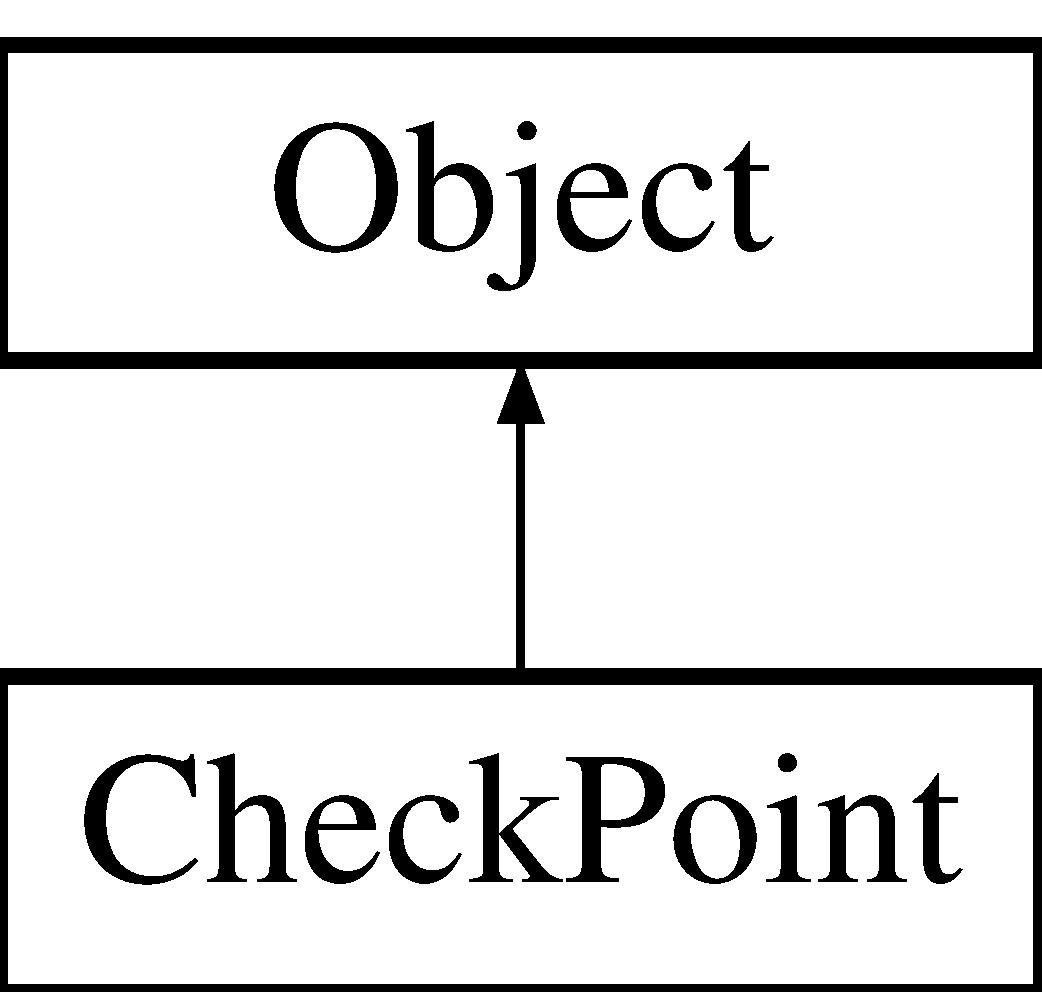
\includegraphics[height=2.000000cm]{classCheckPoint}
\end{center}
\end{figure}
\subsection*{Public Member Functions}
\begin{DoxyCompactItemize}
\item 
\hyperlink{classCheckPoint_a78e714da90f33a69c0413a2f51a988ad}{Check\+Point} ()
\item 
\hyperlink{classCheckPoint_a17653df57b3208932c20fceecf29e7a1}{Check\+Point} (Vector2d pos, int num, int width, int \hyperlink{classObject_aa08efab6c2c6898b1d0d7103076d8674}{angle})
\item 
void \hyperlink{classCheckPoint_abb225b6849ff500b0fe19cdeb927d1b6}{collide} (\hyperlink{classObject}{Object} \&o)
\item 
int \hyperlink{classCheckPoint_a6d0ba1960662239fe108211f3787ca12}{get\+Width} () const
\item 
int \hyperlink{classCheckPoint_a5356134c7455dac27e72dd144642e8ec}{get\+Height} () const
\item 
int \hyperlink{classCheckPoint_a22dca0111d35b2182b825ea6f03f94ed}{get\+Number} () const
\end{DoxyCompactItemize}
\subsection*{Additional Inherited Members}


\subsection{Detailed Description}
A class to follow player\textquotesingle{}s progress in game. Check\+Point-\/object is located in the game area to work as an indicator, whether player has passed a certain point. A integer numbers are set for checkpoints to determint orde in which they have to be visited. 

\subsection{Constructor \& Destructor Documentation}
\hypertarget{classCheckPoint_a78e714da90f33a69c0413a2f51a988ad}{}\label{classCheckPoint_a78e714da90f33a69c0413a2f51a988ad} 
\index{Check\+Point@{Check\+Point}!Check\+Point@{Check\+Point}}
\index{Check\+Point@{Check\+Point}!Check\+Point@{Check\+Point}}
\subsubsection{\texorpdfstring{Check\+Point()}{CheckPoint()}\hspace{0.1cm}{\footnotesize\ttfamily [1/2]}}
{\footnotesize\ttfamily Check\+Point\+::\+Check\+Point (\begin{DoxyParamCaption}{ }\end{DoxyParamCaption})\hspace{0.3cm}{\ttfamily [inline]}}

Constructor \hypertarget{classCheckPoint_a17653df57b3208932c20fceecf29e7a1}{}\label{classCheckPoint_a17653df57b3208932c20fceecf29e7a1} 
\index{Check\+Point@{Check\+Point}!Check\+Point@{Check\+Point}}
\index{Check\+Point@{Check\+Point}!Check\+Point@{Check\+Point}}
\subsubsection{\texorpdfstring{Check\+Point()}{CheckPoint()}\hspace{0.1cm}{\footnotesize\ttfamily [2/2]}}
{\footnotesize\ttfamily Check\+Point\+::\+Check\+Point (\begin{DoxyParamCaption}\item[{Vector2d}]{pos,  }\item[{int}]{num,  }\item[{int}]{width,  }\item[{int}]{angle }\end{DoxyParamCaption})}

Constructor 

\subsection{Member Function Documentation}
\hypertarget{classCheckPoint_abb225b6849ff500b0fe19cdeb927d1b6}{}\label{classCheckPoint_abb225b6849ff500b0fe19cdeb927d1b6} 
\index{Check\+Point@{Check\+Point}!collide@{collide}}
\index{collide@{collide}!Check\+Point@{Check\+Point}}
\subsubsection{\texorpdfstring{collide()}{collide()}}
{\footnotesize\ttfamily void Check\+Point\+::collide (\begin{DoxyParamCaption}\item[{\hyperlink{classObject}{Object} \&}]{o }\end{DoxyParamCaption})\hspace{0.3cm}{\ttfamily [virtual]}}

Returns the order number of checkpoint. Detects if player has passed the checkpoint. 

Implements \hyperlink{classObject}{Object}.

\hypertarget{classCheckPoint_a5356134c7455dac27e72dd144642e8ec}{}\label{classCheckPoint_a5356134c7455dac27e72dd144642e8ec} 
\index{Check\+Point@{Check\+Point}!get\+Height@{get\+Height}}
\index{get\+Height@{get\+Height}!Check\+Point@{Check\+Point}}
\subsubsection{\texorpdfstring{get\+Height()}{getHeight()}}
{\footnotesize\ttfamily int Check\+Point\+::get\+Height (\begin{DoxyParamCaption}{ }\end{DoxyParamCaption}) const\hspace{0.3cm}{\ttfamily [inline]}}

Returns height of checkpoint. \hypertarget{classCheckPoint_a22dca0111d35b2182b825ea6f03f94ed}{}\label{classCheckPoint_a22dca0111d35b2182b825ea6f03f94ed} 
\index{Check\+Point@{Check\+Point}!get\+Number@{get\+Number}}
\index{get\+Number@{get\+Number}!Check\+Point@{Check\+Point}}
\subsubsection{\texorpdfstring{get\+Number()}{getNumber()}}
{\footnotesize\ttfamily int Check\+Point\+::get\+Number (\begin{DoxyParamCaption}{ }\end{DoxyParamCaption}) const\hspace{0.3cm}{\ttfamily [inline]}}

Returns number of checkpoint. \hypertarget{classCheckPoint_a6d0ba1960662239fe108211f3787ca12}{}\label{classCheckPoint_a6d0ba1960662239fe108211f3787ca12} 
\index{Check\+Point@{Check\+Point}!get\+Width@{get\+Width}}
\index{get\+Width@{get\+Width}!Check\+Point@{Check\+Point}}
\subsubsection{\texorpdfstring{get\+Width()}{getWidth()}}
{\footnotesize\ttfamily int Check\+Point\+::get\+Width (\begin{DoxyParamCaption}{ }\end{DoxyParamCaption}) const\hspace{0.3cm}{\ttfamily [inline]}}

Returns width of checkpoint. 

The documentation for this class was generated from the following files\+:\begin{DoxyCompactItemize}
\item 
src/checkpoint.\+hpp\item 
src/checkpoint.\+cpp\end{DoxyCompactItemize}

\hypertarget{classcScreen}{}\section{c\+Screen Class Reference}
\label{classcScreen}\index{c\+Screen@{c\+Screen}}


{\ttfamily \#include $<$c\+Screen.\+hpp$>$}

Inheritance diagram for c\+Screen\+:\begin{figure}[H]
\begin{center}
\leavevmode
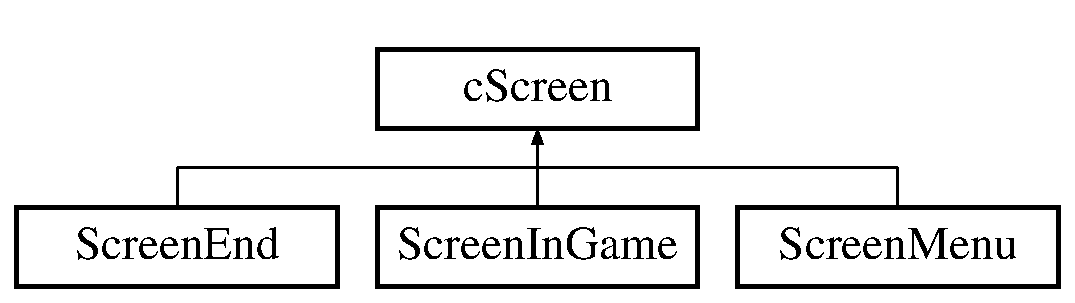
\includegraphics[height=2.000000cm]{classcScreen}
\end{center}
\end{figure}
\subsection*{Public Member Functions}
\begin{DoxyCompactItemize}
\item 
\hyperlink{classcScreen_abb06ae98ccb31bc0fd2174547a10ca0d}{c\+Screen} (std\+::shared\+\_\+ptr$<$ \hyperlink{classGameInfo}{Game\+Info} $>$ info)
\item 
virtual int \hyperlink{classcScreen_a4b4057ffec7ab1492a4de19f9994cac4}{Run} (sf\+::\+Render\+Window \&w)=0
\item 
void \hyperlink{classcScreen_aa741f84e247decd04cb714bc1c33f93d}{set\+\_\+infoptr} (std\+::shared\+\_\+ptr$<$ \hyperlink{classGameInfo}{Game\+Info} $>$ info)
\item 
std\+::shared\+\_\+ptr$<$ \hyperlink{classGameInfo}{Game\+Info} $>$ \hyperlink{classcScreen_a7fea97aa92e8d84dafd9119e9b2545d4}{get\+\_\+infoptr} ()
\end{DoxyCompactItemize}


\subsection{Detailed Description}
A generic class for different scenes or screens inside the game. These include the main menu, the actual game and the end screen. 

\subsection{Constructor \& Destructor Documentation}
\hypertarget{classcScreen_abb06ae98ccb31bc0fd2174547a10ca0d}{}\label{classcScreen_abb06ae98ccb31bc0fd2174547a10ca0d} 
\index{c\+Screen@{c\+Screen}!c\+Screen@{c\+Screen}}
\index{c\+Screen@{c\+Screen}!c\+Screen@{c\+Screen}}
\subsubsection{\texorpdfstring{c\+Screen()}{cScreen()}}
{\footnotesize\ttfamily c\+Screen\+::c\+Screen (\begin{DoxyParamCaption}\item[{std\+::shared\+\_\+ptr$<$ \hyperlink{classGameInfo}{Game\+Info} $>$}]{info }\end{DoxyParamCaption})\hspace{0.3cm}{\ttfamily [inline]}}

Constuctor for the \hyperlink{classcScreen}{c\+Screen} class. 

\subsection{Member Function Documentation}
\hypertarget{classcScreen_a7fea97aa92e8d84dafd9119e9b2545d4}{}\label{classcScreen_a7fea97aa92e8d84dafd9119e9b2545d4} 
\index{c\+Screen@{c\+Screen}!get\+\_\+infoptr@{get\+\_\+infoptr}}
\index{get\+\_\+infoptr@{get\+\_\+infoptr}!c\+Screen@{c\+Screen}}
\subsubsection{\texorpdfstring{get\+\_\+infoptr()}{get\_infoptr()}}
{\footnotesize\ttfamily std\+::shared\+\_\+ptr$<$\hyperlink{classGameInfo}{Game\+Info}$>$ c\+Screen\+::get\+\_\+infoptr (\begin{DoxyParamCaption}{ }\end{DoxyParamCaption})\hspace{0.3cm}{\ttfamily [inline]}}

Returns the shared information class used by the screen. \hypertarget{classcScreen_a4b4057ffec7ab1492a4de19f9994cac4}{}\label{classcScreen_a4b4057ffec7ab1492a4de19f9994cac4} 
\index{c\+Screen@{c\+Screen}!Run@{Run}}
\index{Run@{Run}!c\+Screen@{c\+Screen}}
\subsubsection{\texorpdfstring{Run()}{Run()}}
{\footnotesize\ttfamily virtual int c\+Screen\+::\+Run (\begin{DoxyParamCaption}\item[{sf\+::\+Render\+Window \&}]{w }\end{DoxyParamCaption})\hspace{0.3cm}{\ttfamily [pure virtual]}}

A function to run the scene. The actual gameplay or a menu is completely contained inside this function. 

Implemented in \hyperlink{classScreenMenu_a86af8a6c97bf315bbe88cd2d7ab35abf}{Screen\+Menu}, \hyperlink{classScreenEnd_a3582fcab70f5568fcdc187feeb1383ad}{Screen\+End}, and \hyperlink{classScreenInGame_a55d4f45872f6d488145d1cf71819b960}{Screen\+In\+Game}.

\hypertarget{classcScreen_aa741f84e247decd04cb714bc1c33f93d}{}\label{classcScreen_aa741f84e247decd04cb714bc1c33f93d} 
\index{c\+Screen@{c\+Screen}!set\+\_\+infoptr@{set\+\_\+infoptr}}
\index{set\+\_\+infoptr@{set\+\_\+infoptr}!c\+Screen@{c\+Screen}}
\subsubsection{\texorpdfstring{set\+\_\+infoptr()}{set\_infoptr()}}
{\footnotesize\ttfamily void c\+Screen\+::set\+\_\+infoptr (\begin{DoxyParamCaption}\item[{std\+::shared\+\_\+ptr$<$ \hyperlink{classGameInfo}{Game\+Info} $>$}]{info }\end{DoxyParamCaption})\hspace{0.3cm}{\ttfamily [inline]}}

Sets the shared information class to be used between different screens for the screen. 

The documentation for this class was generated from the following file\+:\begin{DoxyCompactItemize}
\item 
src/c\+Screen.\+hpp\end{DoxyCompactItemize}

\hypertarget{classGameInfo}{}\section{Game\+Info Class Reference}
\label{classGameInfo}\index{Game\+Info@{Game\+Info}}


{\ttfamily \#include $<$gameinfo.\+hpp$>$}

\subsection*{Public Member Functions}
\begin{DoxyCompactItemize}
\item 
\hyperlink{classGameInfo_ae7ded63bd69b007847bd66debaeebc23}{Game\+Info} ()
\item 
void \hyperlink{classGameInfo_a4269ef3313bbf20946f47bbd1c272b6d}{set\+\_\+map\+\_\+path} (std\+::string path)
\item 
std\+::string \hyperlink{classGameInfo_aa9c66670430c8ce52125cea87b6c38a5}{get\+\_\+map\+\_\+path} ()
\item 
void \hyperlink{classGameInfo_aedb1dce53ebf765683a71d57b65c6cef}{set\+\_\+tilemap\+\_\+path} (std\+::string tpath)
\item 
std\+::string \hyperlink{classGameInfo_a4a3618e3691078217e3bec548bcf40cc}{get\+\_\+tilemap\+\_\+path} ()
\item 
void \hyperlink{classGameInfo_a1c348163ac323c617b0306f946d17baa}{set\+\_\+lap\+\_\+total} (int number)
\item 
int \hyperlink{classGameInfo_ab8f5a3a0d1aa460ed0956f211bbc445c}{get\+\_\+lap\+\_\+total} ()
\item 
std\+::shared\+\_\+ptr$<$ \hyperlink{classPlayerInput}{Player\+Input} $>$ \hyperlink{classGameInfo_a4c6bf794f57e952748633c7897d4741d}{get\+Player\+Input} (int p)
\item 
void \hyperlink{classGameInfo_ae4d8a51be4f8d55b177e2fdadb5e4860}{set\+Player\+Input} (\hyperlink{classPlayerInput}{Player\+Input} const \&p, int player)
\end{DoxyCompactItemize}


\subsection{Detailed Description}
Class for storing user-\/defined game settings that is useful to all game screens. 

\subsection{Constructor \& Destructor Documentation}
\hypertarget{classGameInfo_ae7ded63bd69b007847bd66debaeebc23}{}\label{classGameInfo_ae7ded63bd69b007847bd66debaeebc23} 
\index{Game\+Info@{Game\+Info}!Game\+Info@{Game\+Info}}
\index{Game\+Info@{Game\+Info}!Game\+Info@{Game\+Info}}
\subsubsection{\texorpdfstring{Game\+Info()}{GameInfo()}}
{\footnotesize\ttfamily Game\+Info\+::\+Game\+Info (\begin{DoxyParamCaption}{ }\end{DoxyParamCaption})\hspace{0.3cm}{\ttfamily [inline]}}

Constructor 

\subsection{Member Function Documentation}
\hypertarget{classGameInfo_ab8f5a3a0d1aa460ed0956f211bbc445c}{}\label{classGameInfo_ab8f5a3a0d1aa460ed0956f211bbc445c} 
\index{Game\+Info@{Game\+Info}!get\+\_\+lap\+\_\+total@{get\+\_\+lap\+\_\+total}}
\index{get\+\_\+lap\+\_\+total@{get\+\_\+lap\+\_\+total}!Game\+Info@{Game\+Info}}
\subsubsection{\texorpdfstring{get\+\_\+lap\+\_\+total()}{get\_lap\_total()}}
{\footnotesize\ttfamily int Game\+Info\+::get\+\_\+lap\+\_\+total (\begin{DoxyParamCaption}{ }\end{DoxyParamCaption})\hspace{0.3cm}{\ttfamily [inline]}}

Returns the amount of laps in a race. \hypertarget{classGameInfo_aa9c66670430c8ce52125cea87b6c38a5}{}\label{classGameInfo_aa9c66670430c8ce52125cea87b6c38a5} 
\index{Game\+Info@{Game\+Info}!get\+\_\+map\+\_\+path@{get\+\_\+map\+\_\+path}}
\index{get\+\_\+map\+\_\+path@{get\+\_\+map\+\_\+path}!Game\+Info@{Game\+Info}}
\subsubsection{\texorpdfstring{get\+\_\+map\+\_\+path()}{get\_map\_path()}}
{\footnotesize\ttfamily std\+::string Game\+Info\+::get\+\_\+map\+\_\+path (\begin{DoxyParamCaption}{ }\end{DoxyParamCaption})\hspace{0.3cm}{\ttfamily [inline]}}

Returns the current path for mapfile for map generation. \hypertarget{classGameInfo_a4a3618e3691078217e3bec548bcf40cc}{}\label{classGameInfo_a4a3618e3691078217e3bec548bcf40cc} 
\index{Game\+Info@{Game\+Info}!get\+\_\+tilemap\+\_\+path@{get\+\_\+tilemap\+\_\+path}}
\index{get\+\_\+tilemap\+\_\+path@{get\+\_\+tilemap\+\_\+path}!Game\+Info@{Game\+Info}}
\subsubsection{\texorpdfstring{get\+\_\+tilemap\+\_\+path()}{get\_tilemap\_path()}}
{\footnotesize\ttfamily std\+::string Game\+Info\+::get\+\_\+tilemap\+\_\+path (\begin{DoxyParamCaption}{ }\end{DoxyParamCaption})\hspace{0.3cm}{\ttfamily [inline]}}

Returns the current path for tilemap-\/file for map generation. \hypertarget{classGameInfo_a4c6bf794f57e952748633c7897d4741d}{}\label{classGameInfo_a4c6bf794f57e952748633c7897d4741d} 
\index{Game\+Info@{Game\+Info}!get\+Player\+Input@{get\+Player\+Input}}
\index{get\+Player\+Input@{get\+Player\+Input}!Game\+Info@{Game\+Info}}
\subsubsection{\texorpdfstring{get\+Player\+Input()}{getPlayerInput()}}
{\footnotesize\ttfamily std\+::shared\+\_\+ptr$<$\hyperlink{classPlayerInput}{Player\+Input}$>$ Game\+Info\+::get\+Player\+Input (\begin{DoxyParamCaption}\item[{int}]{p }\end{DoxyParamCaption})\hspace{0.3cm}{\ttfamily [inline]}}

Returns Player\+Input-\/object pointer for game controls of player \hypertarget{classGameInfo_a1c348163ac323c617b0306f946d17baa}{}\label{classGameInfo_a1c348163ac323c617b0306f946d17baa} 
\index{Game\+Info@{Game\+Info}!set\+\_\+lap\+\_\+total@{set\+\_\+lap\+\_\+total}}
\index{set\+\_\+lap\+\_\+total@{set\+\_\+lap\+\_\+total}!Game\+Info@{Game\+Info}}
\subsubsection{\texorpdfstring{set\+\_\+lap\+\_\+total()}{set\_lap\_total()}}
{\footnotesize\ttfamily void Game\+Info\+::set\+\_\+lap\+\_\+total (\begin{DoxyParamCaption}\item[{int}]{number }\end{DoxyParamCaption})\hspace{0.3cm}{\ttfamily [inline]}}

Setting the amount of laps in a race. \hypertarget{classGameInfo_a4269ef3313bbf20946f47bbd1c272b6d}{}\label{classGameInfo_a4269ef3313bbf20946f47bbd1c272b6d} 
\index{Game\+Info@{Game\+Info}!set\+\_\+map\+\_\+path@{set\+\_\+map\+\_\+path}}
\index{set\+\_\+map\+\_\+path@{set\+\_\+map\+\_\+path}!Game\+Info@{Game\+Info}}
\subsubsection{\texorpdfstring{set\+\_\+map\+\_\+path()}{set\_map\_path()}}
{\footnotesize\ttfamily void Game\+Info\+::set\+\_\+map\+\_\+path (\begin{DoxyParamCaption}\item[{std\+::string}]{path }\end{DoxyParamCaption})\hspace{0.3cm}{\ttfamily [inline]}}

Setting path of mapfile for map generation. \hypertarget{classGameInfo_aedb1dce53ebf765683a71d57b65c6cef}{}\label{classGameInfo_aedb1dce53ebf765683a71d57b65c6cef} 
\index{Game\+Info@{Game\+Info}!set\+\_\+tilemap\+\_\+path@{set\+\_\+tilemap\+\_\+path}}
\index{set\+\_\+tilemap\+\_\+path@{set\+\_\+tilemap\+\_\+path}!Game\+Info@{Game\+Info}}
\subsubsection{\texorpdfstring{set\+\_\+tilemap\+\_\+path()}{set\_tilemap\_path()}}
{\footnotesize\ttfamily void Game\+Info\+::set\+\_\+tilemap\+\_\+path (\begin{DoxyParamCaption}\item[{std\+::string}]{tpath }\end{DoxyParamCaption})\hspace{0.3cm}{\ttfamily [inline]}}

Setting path for tilemap-\/file for map generation. \hypertarget{classGameInfo_ae4d8a51be4f8d55b177e2fdadb5e4860}{}\label{classGameInfo_ae4d8a51be4f8d55b177e2fdadb5e4860} 
\index{Game\+Info@{Game\+Info}!set\+Player\+Input@{set\+Player\+Input}}
\index{set\+Player\+Input@{set\+Player\+Input}!Game\+Info@{Game\+Info}}
\subsubsection{\texorpdfstring{set\+Player\+Input()}{setPlayerInput()}}
{\footnotesize\ttfamily void Game\+Info\+::set\+Player\+Input (\begin{DoxyParamCaption}\item[{\hyperlink{classPlayerInput}{Player\+Input} const \&}]{p,  }\item[{int}]{player }\end{DoxyParamCaption})\hspace{0.3cm}{\ttfamily [inline]}}

Sets controls for player through Player\+Input-\/object. 

The documentation for this class was generated from the following file\+:\begin{DoxyCompactItemize}
\item 
src/gameinfo.\+hpp\end{DoxyCompactItemize}

\hypertarget{classMap}{}\section{Map Class Reference}
\label{classMap}\index{Map@{Map}}


{\ttfamily \#include $<$map.\+hpp$>$}

\subsection*{Public Member Functions}
\begin{DoxyCompactItemize}
\item 
\hyperlink{classMap_a067a9c057cdf715cbe1484efad9bff27}{Map} (const char $\ast$filename, std\+::shared\+\_\+ptr$<$ \hyperlink{classWorld}{World} $>$)
\item 
void \hyperlink{classMap_accb446c23d408f95e6944fedc742b79f}{set\+Tileset\+Path} (std\+::string const \&s)
\item 
bool \hyperlink{classMap_ae184e30853864425b327b2d5b3cba48b}{load\+Tile\+Map} ()
\item 
void \hyperlink{classMap_a122f46ddff5b5d0b8377425a9a176502}{create\+Walls} (std\+::shared\+\_\+ptr$<$ \hyperlink{classWorld}{World} $>$ w)
\item 
\hyperlink{classTilemap}{Tilemap} \& \hyperlink{classMap_ae1ab0f7883bad946493c6a7f896966f0}{get\+Tilemap} ()
\item 
void \hyperlink{classMap_aa1621a8865fc469ae9c05c08967e4f2c}{draw} (Window \&w)
\item 
int \hyperlink{classMap_a2b09c8875af2efb711fc3a022e70427d}{get\+Height} ()
\item 
int \hyperlink{classMap_afd34d12227676b3cebeed9f5fae2508f}{get\+Width} ()
\item 
sf\+::\+Vector2u \hyperlink{classMap_a97717641214ebe1e105b4afcf412fbb3}{get\+Tile\+Size} ()
\item 
std\+::vector$<$ std\+::shared\+\_\+ptr$<$ \hyperlink{classCheckPoint}{Check\+Point} $>$ $>$ \hyperlink{classMap_a5de4ef4f3422d815f28d8e609964a449}{get\+Check\+Points} ()
\item 
std\+::vector$<$ std\+::shared\+\_\+ptr$<$ \hyperlink{classMine}{Mine} $>$ $>$ \hyperlink{classMap_a5c116280551e3b49145e7d30d392c429}{get\+Mines} ()
\end{DoxyCompactItemize}


\subsection{Detailed Description}
Map-\/class reads game field from a text file in its constructor. Text file consists of characters representing tiles. The text file is assumed to have equally many characters in every row and it ends in newline-\/character 

\subsection{Constructor \& Destructor Documentation}
\hypertarget{classMap_a067a9c057cdf715cbe1484efad9bff27}{}\label{classMap_a067a9c057cdf715cbe1484efad9bff27} 
\index{Map@{Map}!Map@{Map}}
\index{Map@{Map}!Map@{Map}}
\subsubsection{\texorpdfstring{Map()}{Map()}}
{\footnotesize\ttfamily Map\+::\+Map (\begin{DoxyParamCaption}\item[{const char $\ast$}]{filename,  }\item[{std\+::shared\+\_\+ptr$<$ \hyperlink{classWorld}{World} $>$}]{w }\end{DoxyParamCaption})}

Constructor for map. Loads the map from a map file. 

\subsection{Member Function Documentation}
\hypertarget{classMap_a122f46ddff5b5d0b8377425a9a176502}{}\label{classMap_a122f46ddff5b5d0b8377425a9a176502} 
\index{Map@{Map}!create\+Walls@{create\+Walls}}
\index{create\+Walls@{create\+Walls}!Map@{Map}}
\subsubsection{\texorpdfstring{create\+Walls()}{createWalls()}}
{\footnotesize\ttfamily void Map\+::create\+Walls (\begin{DoxyParamCaption}\item[{std\+::shared\+\_\+ptr$<$ \hyperlink{classWorld}{World} $>$}]{w }\end{DoxyParamCaption})}

Creates walls according to map structure. \hypertarget{classMap_aa1621a8865fc469ae9c05c08967e4f2c}{}\label{classMap_aa1621a8865fc469ae9c05c08967e4f2c} 
\index{Map@{Map}!draw@{draw}}
\index{draw@{draw}!Map@{Map}}
\subsubsection{\texorpdfstring{draw()}{draw()}}
{\footnotesize\ttfamily void Map\+::draw (\begin{DoxyParamCaption}\item[{Window \&}]{w }\end{DoxyParamCaption})}

Draws the tilemap. \hypertarget{classMap_a5de4ef4f3422d815f28d8e609964a449}{}\label{classMap_a5de4ef4f3422d815f28d8e609964a449} 
\index{Map@{Map}!get\+Check\+Points@{get\+Check\+Points}}
\index{get\+Check\+Points@{get\+Check\+Points}!Map@{Map}}
\subsubsection{\texorpdfstring{get\+Check\+Points()}{getCheckPoints()}}
{\footnotesize\ttfamily std\+::vector$<$std\+::shared\+\_\+ptr$<$\hyperlink{classCheckPoint}{Check\+Point}$>$ $>$ Map\+::get\+Check\+Points (\begin{DoxyParamCaption}{ }\end{DoxyParamCaption})\hspace{0.3cm}{\ttfamily [inline]}}

Returns the checkpoints as a vector. \hypertarget{classMap_a2b09c8875af2efb711fc3a022e70427d}{}\label{classMap_a2b09c8875af2efb711fc3a022e70427d} 
\index{Map@{Map}!get\+Height@{get\+Height}}
\index{get\+Height@{get\+Height}!Map@{Map}}
\subsubsection{\texorpdfstring{get\+Height()}{getHeight()}}
{\footnotesize\ttfamily int Map\+::get\+Height (\begin{DoxyParamCaption}{ }\end{DoxyParamCaption})\hspace{0.3cm}{\ttfamily [inline]}}

Returns the height of the map. \hypertarget{classMap_a5c116280551e3b49145e7d30d392c429}{}\label{classMap_a5c116280551e3b49145e7d30d392c429} 
\index{Map@{Map}!get\+Mines@{get\+Mines}}
\index{get\+Mines@{get\+Mines}!Map@{Map}}
\subsubsection{\texorpdfstring{get\+Mines()}{getMines()}}
{\footnotesize\ttfamily std\+::vector$<$std\+::shared\+\_\+ptr$<$\hyperlink{classMine}{Mine}$>$ $>$ Map\+::get\+Mines (\begin{DoxyParamCaption}{ }\end{DoxyParamCaption})\hspace{0.3cm}{\ttfamily [inline]}}

Returns the mines of the map as a list \hypertarget{classMap_ae1ab0f7883bad946493c6a7f896966f0}{}\label{classMap_ae1ab0f7883bad946493c6a7f896966f0} 
\index{Map@{Map}!get\+Tilemap@{get\+Tilemap}}
\index{get\+Tilemap@{get\+Tilemap}!Map@{Map}}
\subsubsection{\texorpdfstring{get\+Tilemap()}{getTilemap()}}
{\footnotesize\ttfamily \hyperlink{classTilemap}{Tilemap}\& Map\+::get\+Tilemap (\begin{DoxyParamCaption}{ }\end{DoxyParamCaption})\hspace{0.3cm}{\ttfamily [inline]}}

Returns the tilemap structure. \hypertarget{classMap_a97717641214ebe1e105b4afcf412fbb3}{}\label{classMap_a97717641214ebe1e105b4afcf412fbb3} 
\index{Map@{Map}!get\+Tile\+Size@{get\+Tile\+Size}}
\index{get\+Tile\+Size@{get\+Tile\+Size}!Map@{Map}}
\subsubsection{\texorpdfstring{get\+Tile\+Size()}{getTileSize()}}
{\footnotesize\ttfamily sf\+::\+Vector2u Map\+::get\+Tile\+Size (\begin{DoxyParamCaption}{ }\end{DoxyParamCaption})\hspace{0.3cm}{\ttfamily [inline]}}

Returns the tile size as a vector. \hypertarget{classMap_afd34d12227676b3cebeed9f5fae2508f}{}\label{classMap_afd34d12227676b3cebeed9f5fae2508f} 
\index{Map@{Map}!get\+Width@{get\+Width}}
\index{get\+Width@{get\+Width}!Map@{Map}}
\subsubsection{\texorpdfstring{get\+Width()}{getWidth()}}
{\footnotesize\ttfamily int Map\+::get\+Width (\begin{DoxyParamCaption}{ }\end{DoxyParamCaption})\hspace{0.3cm}{\ttfamily [inline]}}

Returns the idth of the map. \hypertarget{classMap_ae184e30853864425b327b2d5b3cba48b}{}\label{classMap_ae184e30853864425b327b2d5b3cba48b} 
\index{Map@{Map}!load\+Tile\+Map@{load\+Tile\+Map}}
\index{load\+Tile\+Map@{load\+Tile\+Map}!Map@{Map}}
\subsubsection{\texorpdfstring{load\+Tile\+Map()}{loadTileMap()}}
{\footnotesize\ttfamily bool Map\+::load\+Tile\+Map (\begin{DoxyParamCaption}{ }\end{DoxyParamCaption})}

Loads the tilemap according to the map structure and tileset. \hypertarget{classMap_accb446c23d408f95e6944fedc742b79f}{}\label{classMap_accb446c23d408f95e6944fedc742b79f} 
\index{Map@{Map}!set\+Tileset\+Path@{set\+Tileset\+Path}}
\index{set\+Tileset\+Path@{set\+Tileset\+Path}!Map@{Map}}
\subsubsection{\texorpdfstring{set\+Tileset\+Path()}{setTilesetPath()}}
{\footnotesize\ttfamily void Map\+::set\+Tileset\+Path (\begin{DoxyParamCaption}\item[{std\+::string const \&}]{s }\end{DoxyParamCaption})\hspace{0.3cm}{\ttfamily [inline]}}

Sets the path for the tileset path to be used. 

The documentation for this class was generated from the following files\+:\begin{DoxyCompactItemize}
\item 
src/map.\+hpp\item 
src/map.\+cpp\end{DoxyCompactItemize}

\hypertarget{structMenu}{}\section{Menu Struct Reference}
\label{structMenu}\index{Menu@{Menu}}
\subsection*{Public Attributes}
\begin{DoxyCompactItemize}
\item 
\hypertarget{structMenu_a483ad7c1a39c050e33084a03c7769c33}{}\label{structMenu_a483ad7c1a39c050e33084a03c7769c33} 
int {\bfseries main\+\_\+op} =0
\item 
\hypertarget{structMenu_a5b2947be8d42f2323b1f384d8a56d9f8}{}\label{structMenu_a5b2947be8d42f2323b1f384d8a56d9f8} 
int {\bfseries map\+\_\+choice} =0
\item 
\hypertarget{structMenu_aa9d3a590d1b2a6b3e228506bf64e60b4}{}\label{structMenu_aa9d3a590d1b2a6b3e228506bf64e60b4} 
int {\bfseries player\+\_\+choice} =0
\item 
\hypertarget{structMenu_a16fa60b127cf50b1622b743ed271414e}{}\label{structMenu_a16fa60b127cf50b1622b743ed271414e} 
int {\bfseries key} =0
\item 
\hypertarget{structMenu_af2a7cc455d6a726b3cea639ed557976a}{}\label{structMenu_af2a7cc455d6a726b3cea639ed557976a} 
int {\bfseries chosen\+\_\+map} = 0
\item 
\hypertarget{structMenu_a29088eebb78bcb5a4d14c4b81ff53e02}{}\label{structMenu_a29088eebb78bcb5a4d14c4b81ff53e02} 
bool {\bfseries in\+\_\+main} =true
\item 
\hypertarget{structMenu_a70dc6095001f5930485e089ac4f08b42}{}\label{structMenu_a70dc6095001f5930485e089ac4f08b42} 
bool {\bfseries in\+\_\+map} =false
\item 
\hypertarget{structMenu_a99f864aea69c9f9a11871be7d4d96305}{}\label{structMenu_a99f864aea69c9f9a11871be7d4d96305} 
bool {\bfseries in\+\_\+keys} =false
\item 
\hypertarget{structMenu_a68ed738dc56e7fae1c923a8243a67778}{}\label{structMenu_a68ed738dc56e7fae1c923a8243a67778} 
bool {\bfseries in\+\_\+p} = false
\end{DoxyCompactItemize}


\subsection{Detailed Description}
A structure for holding the menu state in. 

The documentation for this struct was generated from the following file\+:\begin{DoxyCompactItemize}
\item 
src/screen\+\_\+menu.\+cpp\end{DoxyCompactItemize}

\hypertarget{classMine}{}\section{Mine Class Reference}
\label{classMine}\index{Mine@{Mine}}


{\ttfamily \#include $<$mine.\+hpp$>$}

Inheritance diagram for Mine\+:\begin{figure}[H]
\begin{center}
\leavevmode
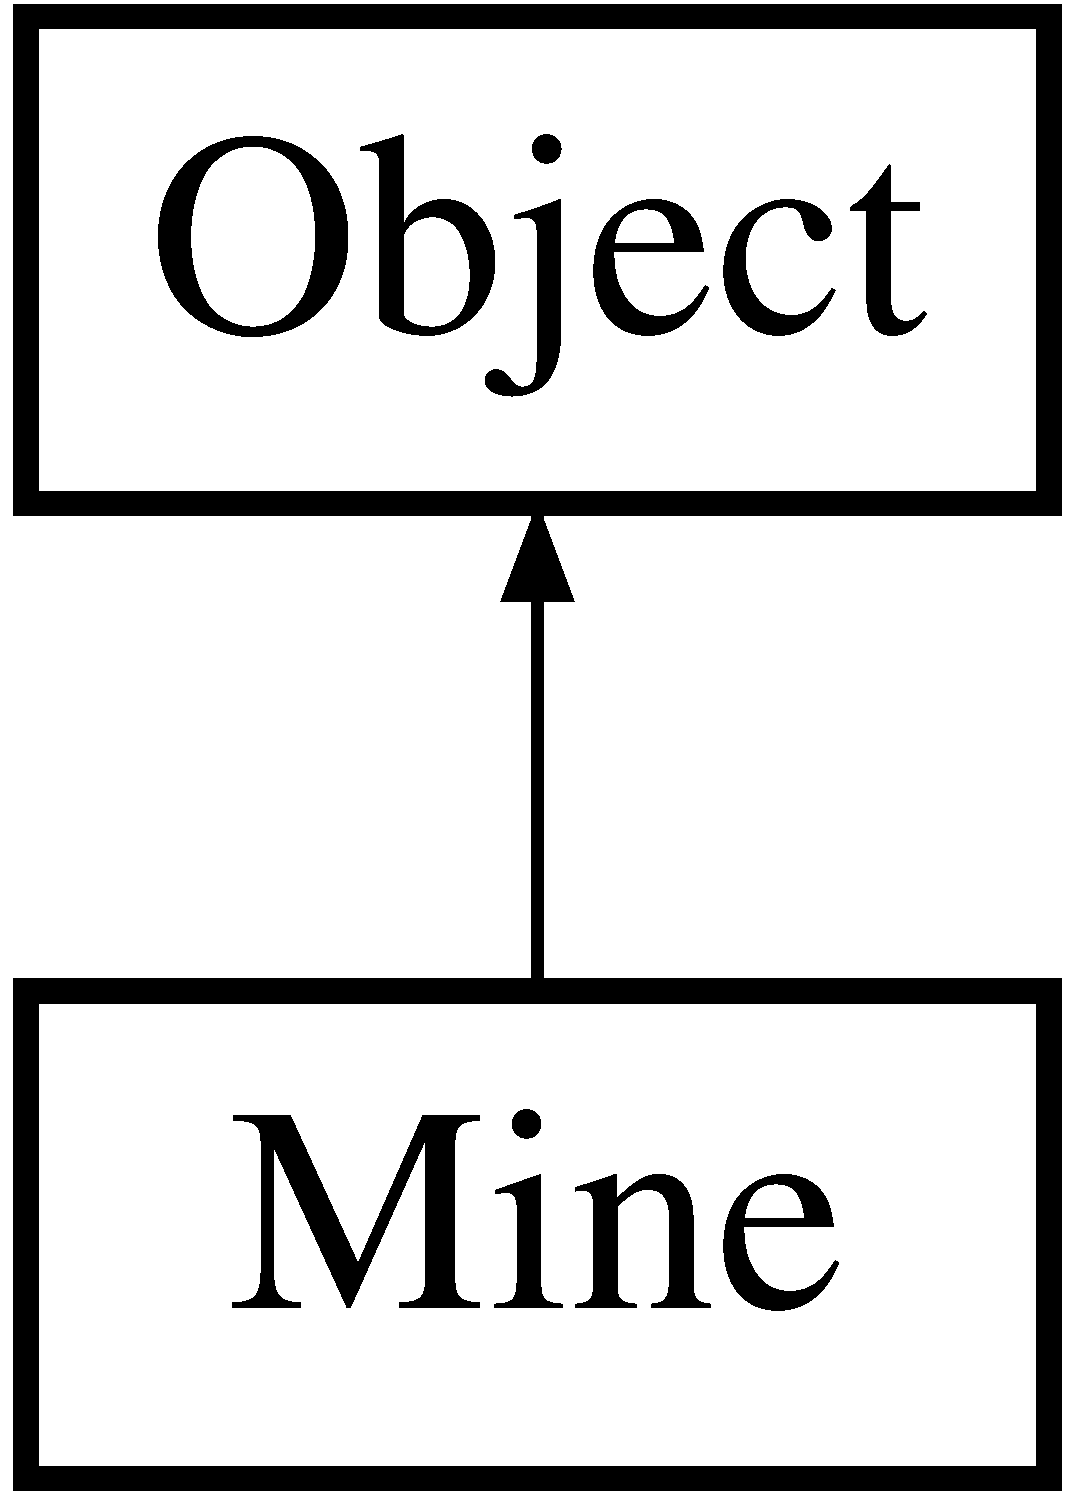
\includegraphics[height=2.000000cm]{classMine}
\end{center}
\end{figure}
\subsection*{Public Member Functions}
\begin{DoxyCompactItemize}
\item 
\hyperlink{classMine_a20441a92f269fcd5f011c2dc40642838}{Mine} (Vector2d, int)
\item 
virtual void \hyperlink{classMine_a8f28428004ed7bd212913d74fc242b3f}{collide} (\hyperlink{classObject}{Object} \&o)
\item 
virtual void \hyperlink{classMine_a56c9fa642d918b17cb20a800e66423cb}{set\+Texture} (sf\+::\+Texture \&)
\item 
void \hyperlink{classMine_a2bb4b5e254618f4ba26816d6774037ed}{update\+State} ()
\item 
bool \hyperlink{classMine_a697a4d8d3872b2155f85ea85347dadda}{is\+Visible} ()
\item 
void \hyperlink{classMine_a8f5acea497c11f9882c74c6e3f3a1554}{set\+Invisible} ()
\item 
void \hyperlink{classMine_a03dc6fa52215e83fe6a1aadc18c9b163}{detonate} ()
\item 
void \hyperlink{classMine_a6305c033929abf20ce4b1c212177d5ec}{draw} (Window \&w)
\item 
sf\+::\+Clock \& \hyperlink{classMine_a21cdef836d82c5fa0bed3125b338181b}{get\+Clock} ()
\end{DoxyCompactItemize}
\subsection*{Additional Inherited Members}


\subsection{Detailed Description}
A class for the sole obstacle in the game. 

\subsection{Constructor \& Destructor Documentation}
\hypertarget{classMine_a20441a92f269fcd5f011c2dc40642838}{}\label{classMine_a20441a92f269fcd5f011c2dc40642838} 
\index{Mine@{Mine}!Mine@{Mine}}
\index{Mine@{Mine}!Mine@{Mine}}
\subsubsection{\texorpdfstring{Mine()}{Mine()}}
{\footnotesize\ttfamily Mine\+::\+Mine (\begin{DoxyParamCaption}\item[{Vector2d}]{pos,  }\item[{int}]{rad }\end{DoxyParamCaption})}

Constructor 

\subsection{Member Function Documentation}
\hypertarget{classMine_a8f28428004ed7bd212913d74fc242b3f}{}\label{classMine_a8f28428004ed7bd212913d74fc242b3f} 
\index{Mine@{Mine}!collide@{collide}}
\index{collide@{collide}!Mine@{Mine}}
\subsubsection{\texorpdfstring{collide()}{collide()}}
{\footnotesize\ttfamily void Mine\+::collide (\begin{DoxyParamCaption}\item[{\hyperlink{classObject}{Object} \&}]{o }\end{DoxyParamCaption})\hspace{0.3cm}{\ttfamily [virtual]}}

Collides the mine with another object. 

Implements \hyperlink{classObject}{Object}.

\hypertarget{classMine_a03dc6fa52215e83fe6a1aadc18c9b163}{}\label{classMine_a03dc6fa52215e83fe6a1aadc18c9b163} 
\index{Mine@{Mine}!detonate@{detonate}}
\index{detonate@{detonate}!Mine@{Mine}}
\subsubsection{\texorpdfstring{detonate()}{detonate()}}
{\footnotesize\ttfamily void Mine\+::detonate (\begin{DoxyParamCaption}{ }\end{DoxyParamCaption})}

Detonates the mine when it comes to contact with a vehicle. \hypertarget{classMine_a6305c033929abf20ce4b1c212177d5ec}{}\label{classMine_a6305c033929abf20ce4b1c212177d5ec} 
\index{Mine@{Mine}!draw@{draw}}
\index{draw@{draw}!Mine@{Mine}}
\subsubsection{\texorpdfstring{draw()}{draw()}}
{\footnotesize\ttfamily void Mine\+::draw (\begin{DoxyParamCaption}\item[{Window \&}]{w }\end{DoxyParamCaption})}

Draws the mine on the window. \hypertarget{classMine_a21cdef836d82c5fa0bed3125b338181b}{}\label{classMine_a21cdef836d82c5fa0bed3125b338181b} 
\index{Mine@{Mine}!get\+Clock@{get\+Clock}}
\index{get\+Clock@{get\+Clock}!Mine@{Mine}}
\subsubsection{\texorpdfstring{get\+Clock()}{getClock()}}
{\footnotesize\ttfamily sf\+::\+Clock\& Mine\+::get\+Clock (\begin{DoxyParamCaption}{ }\end{DoxyParamCaption})}

Returns the clock that controls the cooldown of the mine. \hypertarget{classMine_a697a4d8d3872b2155f85ea85347dadda}{}\label{classMine_a697a4d8d3872b2155f85ea85347dadda} 
\index{Mine@{Mine}!is\+Visible@{is\+Visible}}
\index{is\+Visible@{is\+Visible}!Mine@{Mine}}
\subsubsection{\texorpdfstring{is\+Visible()}{isVisible()}}
{\footnotesize\ttfamily bool Mine\+::is\+Visible (\begin{DoxyParamCaption}{ }\end{DoxyParamCaption})}

Checks whether the mine is inactive or not. \hypertarget{classMine_a8f5acea497c11f9882c74c6e3f3a1554}{}\label{classMine_a8f5acea497c11f9882c74c6e3f3a1554} 
\index{Mine@{Mine}!set\+Invisible@{set\+Invisible}}
\index{set\+Invisible@{set\+Invisible}!Mine@{Mine}}
\subsubsection{\texorpdfstring{set\+Invisible()}{setInvisible()}}
{\footnotesize\ttfamily void Mine\+::set\+Invisible (\begin{DoxyParamCaption}{ }\end{DoxyParamCaption})}

Sets the mine inactive. \hypertarget{classMine_a56c9fa642d918b17cb20a800e66423cb}{}\label{classMine_a56c9fa642d918b17cb20a800e66423cb} 
\index{Mine@{Mine}!set\+Texture@{set\+Texture}}
\index{set\+Texture@{set\+Texture}!Mine@{Mine}}
\subsubsection{\texorpdfstring{set\+Texture()}{setTexture()}}
{\footnotesize\ttfamily void Mine\+::set\+Texture (\begin{DoxyParamCaption}\item[{sf\+::\+Texture \&}]{tex }\end{DoxyParamCaption})\hspace{0.3cm}{\ttfamily [virtual]}}

Sets the texture for the mine. 

Reimplemented from \hyperlink{classObject_a3b23ad400ac8a7133fb470daa4e67467}{Object}.

\hypertarget{classMine_a2bb4b5e254618f4ba26816d6774037ed}{}\label{classMine_a2bb4b5e254618f4ba26816d6774037ed} 
\index{Mine@{Mine}!update\+State@{update\+State}}
\index{update\+State@{update\+State}!Mine@{Mine}}
\subsubsection{\texorpdfstring{update\+State()}{updateState()}}
{\footnotesize\ttfamily void Mine\+::update\+State (\begin{DoxyParamCaption}{ }\end{DoxyParamCaption})}

Updates the mine\textquotesingle{}s state, including its position. 

The documentation for this class was generated from the following files\+:\begin{DoxyCompactItemize}
\item 
src/mine.\+hpp\item 
src/mine.\+cpp\end{DoxyCompactItemize}

\hypertarget{classObject}{}\section{Object Class Reference}
\label{classObject}\index{Object@{Object}}


{\ttfamily \#include $<$object.\+hpp$>$}

Inheritance diagram for Object\+:\begin{figure}[H]
\begin{center}
\leavevmode
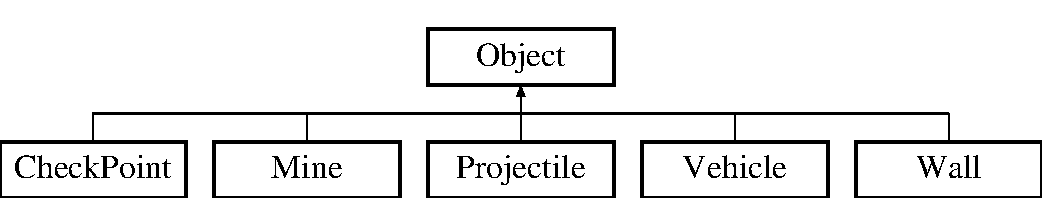
\includegraphics[height=2.000000cm]{classObject}
\end{center}
\end{figure}
\subsection*{Public Member Functions}
\begin{DoxyCompactItemize}
\item 
const Vector2d \& \hyperlink{classObject_ab498ce65ce8cb69bb806081e65f19cd6}{get\+Position} () const
\item 
void \hyperlink{classObject_a03d47d414e9638846de79b4f15cda00f}{set\+Position} (Vector2d const \&p)
\item 
const Vector2d \& \hyperlink{classObject_a0c3105820f784f07a6d20e019a8311a6}{get\+Speed} () const
\item 
void \hyperlink{classObject_a34421c57b89f3c9c6e0de44c98469585}{set\+Speed} (Vector2d const \&s)
\item 
virtual void \hyperlink{classObject_a3b23ad400ac8a7133fb470daa4e67467}{set\+Texture} (sf\+::\+Texture \&)
\item 
double \hyperlink{classObject_ac53341c11f7435033434bc3b6c908f0c}{get\+Mass} () const
\item 
void \hyperlink{classObject_a07221bb6a7c823b993005f8a0d3cd7a1}{set\+Mass} (double const \&m)
\item 
double \hyperlink{classObject_a9958ed5111be9373ef97cb20d00b625f}{get\+Angle} () const
\item 
void \hyperlink{classObject_a7e69ebba88f99341baf4d046be6493f1}{set\+Angle} (double const \&a)
\item 
sf\+::\+Sprite \hyperlink{classObject_add7c5a02624a3dbdf856517b18fce61f}{get\+Sprite} () const
\item 
void \hyperlink{classObject_a4da149ed27dfef04d62cb2fa6315af1c}{draw} (Window \&w)
\item 
double \hyperlink{classObject_a3d76eb87b30cfd6c9812a2d85a26b187}{get\+Radius} () const
\end{DoxyCompactItemize}
\subsection*{Protected Member Functions}
\begin{DoxyCompactItemize}
\item 
bool \hyperlink{classObject_a4651b3e887145345efc01e98bb9e7b15}{collides} (\hyperlink{classObject}{Object} const \&o) const
\item 
bool \hyperlink{classObject_a9f3dd05fa465ed26bcb89a92dd25190c}{collides} (\hyperlink{classWall}{Wall} const \&w) const
\item 
bool \hyperlink{classObject_a6e41ad759709da8f973419a57c5e7a1c}{collides} (\hyperlink{classCheckPoint}{Check\+Point} const \&cp) const
\item 
\hypertarget{classObject_a026ddef458c358eef33f631c4db42172}{}\label{classObject_a026ddef458c358eef33f631c4db42172} 
virtual void {\bfseries collide} (\hyperlink{classObject}{Object} \&o)=0
\end{DoxyCompactItemize}
\subsection*{Protected Attributes}
\begin{DoxyCompactItemize}
\item 
Vector2d \hyperlink{classObject_ab77f145878370ab7b92f067432dc375c}{position}
\item 
Vector2d \hyperlink{classObject_a740762c9fe723eda94fe82862a8fa200}{speed}
\item 
double \hyperlink{classObject_aa08efab6c2c6898b1d0d7103076d8674}{angle}
\item 
double \hyperlink{classObject_abbd565f533683168a39d703f3b5c6bae}{mass}
\item 
double \hyperlink{classObject_aacfbf5151daad699c60efc27fb702406}{radius}
\item 
sf\+::\+Sprite \hyperlink{classObject_a65be09abc56e93e0154c3a0e37f97579}{sprite}
\item 
sf\+::\+Texture \hyperlink{classObject_a8abc6192982ee39b2dc9d9b05cc155ee}{texture}
\end{DoxyCompactItemize}


\subsection{Detailed Description}
Generic class for game objects, such players, checkpoints and projectiles. 

\subsection{Member Function Documentation}
\hypertarget{classObject_a4651b3e887145345efc01e98bb9e7b15}{}\label{classObject_a4651b3e887145345efc01e98bb9e7b15} 
\index{Object@{Object}!collides@{collides}}
\index{collides@{collides}!Object@{Object}}
\subsubsection{\texorpdfstring{collides()}{collides()}\hspace{0.1cm}{\footnotesize\ttfamily [1/3]}}
{\footnotesize\ttfamily bool Object\+::collides (\begin{DoxyParamCaption}\item[{\hyperlink{classObject}{Object} const \&}]{o }\end{DoxyParamCaption}) const\hspace{0.3cm}{\ttfamily [protected]}}

Checks if an object collides with another object. \hypertarget{classObject_a9f3dd05fa465ed26bcb89a92dd25190c}{}\label{classObject_a9f3dd05fa465ed26bcb89a92dd25190c} 
\index{Object@{Object}!collides@{collides}}
\index{collides@{collides}!Object@{Object}}
\subsubsection{\texorpdfstring{collides()}{collides()}\hspace{0.1cm}{\footnotesize\ttfamily [2/3]}}
{\footnotesize\ttfamily bool Object\+::collides (\begin{DoxyParamCaption}\item[{\hyperlink{classWall}{Wall} const \&}]{w }\end{DoxyParamCaption}) const\hspace{0.3cm}{\ttfamily [protected]}}

Checks if an object collides with a wall. \hypertarget{classObject_a6e41ad759709da8f973419a57c5e7a1c}{}\label{classObject_a6e41ad759709da8f973419a57c5e7a1c} 
\index{Object@{Object}!collides@{collides}}
\index{collides@{collides}!Object@{Object}}
\subsubsection{\texorpdfstring{collides()}{collides()}\hspace{0.1cm}{\footnotesize\ttfamily [3/3]}}
{\footnotesize\ttfamily bool Object\+::collides (\begin{DoxyParamCaption}\item[{\hyperlink{classCheckPoint}{Check\+Point} const \&}]{cp }\end{DoxyParamCaption}) const\hspace{0.3cm}{\ttfamily [protected]}}

checks if an object collides with a map checkpoint. \hypertarget{classObject_a4da149ed27dfef04d62cb2fa6315af1c}{}\label{classObject_a4da149ed27dfef04d62cb2fa6315af1c} 
\index{Object@{Object}!draw@{draw}}
\index{draw@{draw}!Object@{Object}}
\subsubsection{\texorpdfstring{draw()}{draw()}}
{\footnotesize\ttfamily void Object\+::draw (\begin{DoxyParamCaption}\item[{Window \&}]{w }\end{DoxyParamCaption})}

Draws an object on a window. \hypertarget{classObject_a9958ed5111be9373ef97cb20d00b625f}{}\label{classObject_a9958ed5111be9373ef97cb20d00b625f} 
\index{Object@{Object}!get\+Angle@{get\+Angle}}
\index{get\+Angle@{get\+Angle}!Object@{Object}}
\subsubsection{\texorpdfstring{get\+Angle()}{getAngle()}}
{\footnotesize\ttfamily double Object\+::get\+Angle (\begin{DoxyParamCaption}{ }\end{DoxyParamCaption}) const}

Returns the angle of an object in degrees. \hypertarget{classObject_ac53341c11f7435033434bc3b6c908f0c}{}\label{classObject_ac53341c11f7435033434bc3b6c908f0c} 
\index{Object@{Object}!get\+Mass@{get\+Mass}}
\index{get\+Mass@{get\+Mass}!Object@{Object}}
\subsubsection{\texorpdfstring{get\+Mass()}{getMass()}}
{\footnotesize\ttfamily double Object\+::get\+Mass (\begin{DoxyParamCaption}{ }\end{DoxyParamCaption}) const}

Returns the mass of an object. \hypertarget{classObject_ab498ce65ce8cb69bb806081e65f19cd6}{}\label{classObject_ab498ce65ce8cb69bb806081e65f19cd6} 
\index{Object@{Object}!get\+Position@{get\+Position}}
\index{get\+Position@{get\+Position}!Object@{Object}}
\subsubsection{\texorpdfstring{get\+Position()}{getPosition()}}
{\footnotesize\ttfamily const Vector2d \& Object\+::get\+Position (\begin{DoxyParamCaption}{ }\end{DoxyParamCaption}) const}

Returns the objects position in pixels as a 2d vector. \hypertarget{classObject_a3d76eb87b30cfd6c9812a2d85a26b187}{}\label{classObject_a3d76eb87b30cfd6c9812a2d85a26b187} 
\index{Object@{Object}!get\+Radius@{get\+Radius}}
\index{get\+Radius@{get\+Radius}!Object@{Object}}
\subsubsection{\texorpdfstring{get\+Radius()}{getRadius()}}
{\footnotesize\ttfamily double Object\+::get\+Radius (\begin{DoxyParamCaption}{ }\end{DoxyParamCaption}) const}

Returns the radius of an object. \hypertarget{classObject_a0c3105820f784f07a6d20e019a8311a6}{}\label{classObject_a0c3105820f784f07a6d20e019a8311a6} 
\index{Object@{Object}!get\+Speed@{get\+Speed}}
\index{get\+Speed@{get\+Speed}!Object@{Object}}
\subsubsection{\texorpdfstring{get\+Speed()}{getSpeed()}}
{\footnotesize\ttfamily const Vector2d \& Object\+::get\+Speed (\begin{DoxyParamCaption}{ }\end{DoxyParamCaption}) const}

Returns the speed of an object. \hypertarget{classObject_add7c5a02624a3dbdf856517b18fce61f}{}\label{classObject_add7c5a02624a3dbdf856517b18fce61f} 
\index{Object@{Object}!get\+Sprite@{get\+Sprite}}
\index{get\+Sprite@{get\+Sprite}!Object@{Object}}
\subsubsection{\texorpdfstring{get\+Sprite()}{getSprite()}}
{\footnotesize\ttfamily sf\+::\+Sprite Object\+::get\+Sprite (\begin{DoxyParamCaption}{ }\end{DoxyParamCaption}) const}

Returns the sprite of an object. \hypertarget{classObject_a7e69ebba88f99341baf4d046be6493f1}{}\label{classObject_a7e69ebba88f99341baf4d046be6493f1} 
\index{Object@{Object}!set\+Angle@{set\+Angle}}
\index{set\+Angle@{set\+Angle}!Object@{Object}}
\subsubsection{\texorpdfstring{set\+Angle()}{setAngle()}}
{\footnotesize\ttfamily void Object\+::set\+Angle (\begin{DoxyParamCaption}\item[{double const \&}]{a }\end{DoxyParamCaption})}

Sets the angle of an object in degrees. \hypertarget{classObject_a07221bb6a7c823b993005f8a0d3cd7a1}{}\label{classObject_a07221bb6a7c823b993005f8a0d3cd7a1} 
\index{Object@{Object}!set\+Mass@{set\+Mass}}
\index{set\+Mass@{set\+Mass}!Object@{Object}}
\subsubsection{\texorpdfstring{set\+Mass()}{setMass()}}
{\footnotesize\ttfamily void Object\+::set\+Mass (\begin{DoxyParamCaption}\item[{double const \&}]{m }\end{DoxyParamCaption})}

Sets the mass of an object. \hypertarget{classObject_a03d47d414e9638846de79b4f15cda00f}{}\label{classObject_a03d47d414e9638846de79b4f15cda00f} 
\index{Object@{Object}!set\+Position@{set\+Position}}
\index{set\+Position@{set\+Position}!Object@{Object}}
\subsubsection{\texorpdfstring{set\+Position()}{setPosition()}}
{\footnotesize\ttfamily void Object\+::set\+Position (\begin{DoxyParamCaption}\item[{Vector2d const \&}]{p }\end{DoxyParamCaption})}

Sets the position of an object. \hypertarget{classObject_a34421c57b89f3c9c6e0de44c98469585}{}\label{classObject_a34421c57b89f3c9c6e0de44c98469585} 
\index{Object@{Object}!set\+Speed@{set\+Speed}}
\index{set\+Speed@{set\+Speed}!Object@{Object}}
\subsubsection{\texorpdfstring{set\+Speed()}{setSpeed()}}
{\footnotesize\ttfamily void Object\+::set\+Speed (\begin{DoxyParamCaption}\item[{Vector2d const \&}]{s }\end{DoxyParamCaption})}

Sets the speed of an object. \hypertarget{classObject_a3b23ad400ac8a7133fb470daa4e67467}{}\label{classObject_a3b23ad400ac8a7133fb470daa4e67467} 
\index{Object@{Object}!set\+Texture@{set\+Texture}}
\index{set\+Texture@{set\+Texture}!Object@{Object}}
\subsubsection{\texorpdfstring{set\+Texture()}{setTexture()}}
{\footnotesize\ttfamily virtual void Object\+::set\+Texture (\begin{DoxyParamCaption}\item[{sf\+::\+Texture \&}]{ }\end{DoxyParamCaption})\hspace{0.3cm}{\ttfamily [inline]}, {\ttfamily [virtual]}}

virtual function for the setting of a texture. 

Reimplemented in \hyperlink{classMine_a56c9fa642d918b17cb20a800e66423cb}{Mine}.



\subsection{Member Data Documentation}
\hypertarget{classObject_aa08efab6c2c6898b1d0d7103076d8674}{}\label{classObject_aa08efab6c2c6898b1d0d7103076d8674} 
\index{Object@{Object}!angle@{angle}}
\index{angle@{angle}!Object@{Object}}
\subsubsection{\texorpdfstring{angle}{angle}}
{\footnotesize\ttfamily double Object\+::angle\hspace{0.3cm}{\ttfamily [protected]}}

Angle of the object in degrees. \hypertarget{classObject_abbd565f533683168a39d703f3b5c6bae}{}\label{classObject_abbd565f533683168a39d703f3b5c6bae} 
\index{Object@{Object}!mass@{mass}}
\index{mass@{mass}!Object@{Object}}
\subsubsection{\texorpdfstring{mass}{mass}}
{\footnotesize\ttfamily double Object\+::mass\hspace{0.3cm}{\ttfamily [protected]}}

Mass of the object. \hypertarget{classObject_ab77f145878370ab7b92f067432dc375c}{}\label{classObject_ab77f145878370ab7b92f067432dc375c} 
\index{Object@{Object}!position@{position}}
\index{position@{position}!Object@{Object}}
\subsubsection{\texorpdfstring{position}{position}}
{\footnotesize\ttfamily Vector2d Object\+::position\hspace{0.3cm}{\ttfamily [protected]}}

Position of the object as a vector. \hypertarget{classObject_aacfbf5151daad699c60efc27fb702406}{}\label{classObject_aacfbf5151daad699c60efc27fb702406} 
\index{Object@{Object}!radius@{radius}}
\index{radius@{radius}!Object@{Object}}
\subsubsection{\texorpdfstring{radius}{radius}}
{\footnotesize\ttfamily double Object\+::radius\hspace{0.3cm}{\ttfamily [protected]}}

Radius of the object. \hypertarget{classObject_a740762c9fe723eda94fe82862a8fa200}{}\label{classObject_a740762c9fe723eda94fe82862a8fa200} 
\index{Object@{Object}!speed@{speed}}
\index{speed@{speed}!Object@{Object}}
\subsubsection{\texorpdfstring{speed}{speed}}
{\footnotesize\ttfamily Vector2d Object\+::speed\hspace{0.3cm}{\ttfamily [protected]}}

Speed of the object as a vector. \hypertarget{classObject_a65be09abc56e93e0154c3a0e37f97579}{}\label{classObject_a65be09abc56e93e0154c3a0e37f97579} 
\index{Object@{Object}!sprite@{sprite}}
\index{sprite@{sprite}!Object@{Object}}
\subsubsection{\texorpdfstring{sprite}{sprite}}
{\footnotesize\ttfamily sf\+::\+Sprite Object\+::sprite\hspace{0.3cm}{\ttfamily [protected]}}

Sprite of the object. \hypertarget{classObject_a8abc6192982ee39b2dc9d9b05cc155ee}{}\label{classObject_a8abc6192982ee39b2dc9d9b05cc155ee} 
\index{Object@{Object}!texture@{texture}}
\index{texture@{texture}!Object@{Object}}
\subsubsection{\texorpdfstring{texture}{texture}}
{\footnotesize\ttfamily sf\+::\+Texture Object\+::texture\hspace{0.3cm}{\ttfamily [protected]}}

Texture of the object. 

The documentation for this class was generated from the following files\+:\begin{DoxyCompactItemize}
\item 
src/object.\+hpp\item 
src/object.\+cpp\end{DoxyCompactItemize}

\hypertarget{classPlayerInput}{}\section{Player\+Input Class Reference}
\label{classPlayerInput}\index{Player\+Input@{Player\+Input}}


{\ttfamily \#include $<$playerinput.\+hpp$>$}

\subsection*{Public Member Functions}
\begin{DoxyCompactItemize}
\item 
sf\+::\+Keyboard\+::\+Key \hyperlink{classPlayerInput_a349bd5b6c64f170e88b409f2ce5384f3}{get\+Key\+Up} () const
\item 
void \hyperlink{classPlayerInput_ac28c127fd9a00d9983061057548e8d6b}{set\+Key\+Up} (sf\+::\+Keyboard\+::\+Key k)
\item 
sf\+::\+Keyboard\+::\+Key \hyperlink{classPlayerInput_a5186c06d0e7f5553787f60ba5673d0cb}{get\+Key\+Down} () const
\item 
void \hyperlink{classPlayerInput_aef9ce827dd9c97f7657e6a53188d63ae}{set\+Key\+Down} (sf\+::\+Keyboard\+::\+Key k)
\item 
sf\+::\+Keyboard\+::\+Key \hyperlink{classPlayerInput_aa046d257f45b62228d6de973d120f391}{get\+Key\+Right} () const
\item 
void \hyperlink{classPlayerInput_a5f09a7c77ae9c20f8246be5eda9856b8}{set\+Key\+Right} (sf\+::\+Keyboard\+::\+Key k)
\item 
sf\+::\+Keyboard\+::\+Key \hyperlink{classPlayerInput_a010e08e15347be2891655f8687a37dcb}{get\+Key\+Left} () const
\item 
void \hyperlink{classPlayerInput_a3025371e730b36a0ae1cb6ec7391e7f8}{set\+Key\+Left} (sf\+::\+Keyboard\+::\+Key k)
\item 
sf\+::\+Keyboard\+::\+Key \hyperlink{classPlayerInput_aa63de3b5eb312b8e5be58dc3b9ef8648}{get\+Key\+Shoot} () const
\item 
void \hyperlink{classPlayerInput_aeae833b00ec51fb096811a828b4b6e9b}{set\+Key\+Shoot} (sf\+::\+Keyboard\+::\+Key k)
\item 
bool \hyperlink{classPlayerInput_a2cd0fa6c370da0294219c326d251ba75}{Up} ()
\item 
bool \hyperlink{classPlayerInput_a0ddb6706f436832085c6e857ce1b6876}{Down} ()
\item 
bool \hyperlink{classPlayerInput_a7b1446e7877945b3361ea2775b182725}{Left} ()
\item 
bool \hyperlink{classPlayerInput_aa9aa970dfc19149b06ff07d956a1cd93}{Right} ()
\item 
bool \hyperlink{classPlayerInput_a5acff106260290af275b0559f8f72dd9}{Shoot} ()
\end{DoxyCompactItemize}


\subsection{Detailed Description}
A class for taking input from player. 

\subsection{Member Function Documentation}
\hypertarget{classPlayerInput_a0ddb6706f436832085c6e857ce1b6876}{}\label{classPlayerInput_a0ddb6706f436832085c6e857ce1b6876} 
\index{Player\+Input@{Player\+Input}!Down@{Down}}
\index{Down@{Down}!Player\+Input@{Player\+Input}}
\subsubsection{\texorpdfstring{Down()}{Down()}}
{\footnotesize\ttfamily bool Player\+Input\+::\+Down (\begin{DoxyParamCaption}{ }\end{DoxyParamCaption})}

Returns whether player is pressing his designated down key. \hypertarget{classPlayerInput_a5186c06d0e7f5553787f60ba5673d0cb}{}\label{classPlayerInput_a5186c06d0e7f5553787f60ba5673d0cb} 
\index{Player\+Input@{Player\+Input}!get\+Key\+Down@{get\+Key\+Down}}
\index{get\+Key\+Down@{get\+Key\+Down}!Player\+Input@{Player\+Input}}
\subsubsection{\texorpdfstring{get\+Key\+Down()}{getKeyDown()}}
{\footnotesize\ttfamily sf\+::\+Keyboard\+::\+Key Player\+Input\+::get\+Key\+Down (\begin{DoxyParamCaption}{ }\end{DoxyParamCaption}) const}

Returns player down key value. \hypertarget{classPlayerInput_a010e08e15347be2891655f8687a37dcb}{}\label{classPlayerInput_a010e08e15347be2891655f8687a37dcb} 
\index{Player\+Input@{Player\+Input}!get\+Key\+Left@{get\+Key\+Left}}
\index{get\+Key\+Left@{get\+Key\+Left}!Player\+Input@{Player\+Input}}
\subsubsection{\texorpdfstring{get\+Key\+Left()}{getKeyLeft()}}
{\footnotesize\ttfamily sf\+::\+Keyboard\+::\+Key Player\+Input\+::get\+Key\+Left (\begin{DoxyParamCaption}{ }\end{DoxyParamCaption}) const}

Returns player left key value. \hypertarget{classPlayerInput_aa046d257f45b62228d6de973d120f391}{}\label{classPlayerInput_aa046d257f45b62228d6de973d120f391} 
\index{Player\+Input@{Player\+Input}!get\+Key\+Right@{get\+Key\+Right}}
\index{get\+Key\+Right@{get\+Key\+Right}!Player\+Input@{Player\+Input}}
\subsubsection{\texorpdfstring{get\+Key\+Right()}{getKeyRight()}}
{\footnotesize\ttfamily sf\+::\+Keyboard\+::\+Key Player\+Input\+::get\+Key\+Right (\begin{DoxyParamCaption}{ }\end{DoxyParamCaption}) const}

Returns player right key value. \hypertarget{classPlayerInput_aa63de3b5eb312b8e5be58dc3b9ef8648}{}\label{classPlayerInput_aa63de3b5eb312b8e5be58dc3b9ef8648} 
\index{Player\+Input@{Player\+Input}!get\+Key\+Shoot@{get\+Key\+Shoot}}
\index{get\+Key\+Shoot@{get\+Key\+Shoot}!Player\+Input@{Player\+Input}}
\subsubsection{\texorpdfstring{get\+Key\+Shoot()}{getKeyShoot()}}
{\footnotesize\ttfamily sf\+::\+Keyboard\+::\+Key Player\+Input\+::get\+Key\+Shoot (\begin{DoxyParamCaption}{ }\end{DoxyParamCaption}) const}

Returns player shoot key value. \hypertarget{classPlayerInput_a349bd5b6c64f170e88b409f2ce5384f3}{}\label{classPlayerInput_a349bd5b6c64f170e88b409f2ce5384f3} 
\index{Player\+Input@{Player\+Input}!get\+Key\+Up@{get\+Key\+Up}}
\index{get\+Key\+Up@{get\+Key\+Up}!Player\+Input@{Player\+Input}}
\subsubsection{\texorpdfstring{get\+Key\+Up()}{getKeyUp()}}
{\footnotesize\ttfamily sf\+::\+Keyboard\+::\+Key Player\+Input\+::get\+Key\+Up (\begin{DoxyParamCaption}{ }\end{DoxyParamCaption}) const}

Returns player up key value. \hypertarget{classPlayerInput_a7b1446e7877945b3361ea2775b182725}{}\label{classPlayerInput_a7b1446e7877945b3361ea2775b182725} 
\index{Player\+Input@{Player\+Input}!Left@{Left}}
\index{Left@{Left}!Player\+Input@{Player\+Input}}
\subsubsection{\texorpdfstring{Left()}{Left()}}
{\footnotesize\ttfamily bool Player\+Input\+::\+Left (\begin{DoxyParamCaption}{ }\end{DoxyParamCaption})}

Returns whether player is pressing his designated left key. \hypertarget{classPlayerInput_aa9aa970dfc19149b06ff07d956a1cd93}{}\label{classPlayerInput_aa9aa970dfc19149b06ff07d956a1cd93} 
\index{Player\+Input@{Player\+Input}!Right@{Right}}
\index{Right@{Right}!Player\+Input@{Player\+Input}}
\subsubsection{\texorpdfstring{Right()}{Right()}}
{\footnotesize\ttfamily bool Player\+Input\+::\+Right (\begin{DoxyParamCaption}{ }\end{DoxyParamCaption})}

Returns whether player is pressing his designated right key. \hypertarget{classPlayerInput_aef9ce827dd9c97f7657e6a53188d63ae}{}\label{classPlayerInput_aef9ce827dd9c97f7657e6a53188d63ae} 
\index{Player\+Input@{Player\+Input}!set\+Key\+Down@{set\+Key\+Down}}
\index{set\+Key\+Down@{set\+Key\+Down}!Player\+Input@{Player\+Input}}
\subsubsection{\texorpdfstring{set\+Key\+Down()}{setKeyDown()}}
{\footnotesize\ttfamily void Player\+Input\+::set\+Key\+Down (\begin{DoxyParamCaption}\item[{sf\+::\+Keyboard\+::\+Key}]{k }\end{DoxyParamCaption})}

Sets player down key value. \hypertarget{classPlayerInput_a3025371e730b36a0ae1cb6ec7391e7f8}{}\label{classPlayerInput_a3025371e730b36a0ae1cb6ec7391e7f8} 
\index{Player\+Input@{Player\+Input}!set\+Key\+Left@{set\+Key\+Left}}
\index{set\+Key\+Left@{set\+Key\+Left}!Player\+Input@{Player\+Input}}
\subsubsection{\texorpdfstring{set\+Key\+Left()}{setKeyLeft()}}
{\footnotesize\ttfamily void Player\+Input\+::set\+Key\+Left (\begin{DoxyParamCaption}\item[{sf\+::\+Keyboard\+::\+Key}]{k }\end{DoxyParamCaption})}

Sets player left key value. \hypertarget{classPlayerInput_a5f09a7c77ae9c20f8246be5eda9856b8}{}\label{classPlayerInput_a5f09a7c77ae9c20f8246be5eda9856b8} 
\index{Player\+Input@{Player\+Input}!set\+Key\+Right@{set\+Key\+Right}}
\index{set\+Key\+Right@{set\+Key\+Right}!Player\+Input@{Player\+Input}}
\subsubsection{\texorpdfstring{set\+Key\+Right()}{setKeyRight()}}
{\footnotesize\ttfamily void Player\+Input\+::set\+Key\+Right (\begin{DoxyParamCaption}\item[{sf\+::\+Keyboard\+::\+Key}]{k }\end{DoxyParamCaption})}

Sets player right key value. \hypertarget{classPlayerInput_aeae833b00ec51fb096811a828b4b6e9b}{}\label{classPlayerInput_aeae833b00ec51fb096811a828b4b6e9b} 
\index{Player\+Input@{Player\+Input}!set\+Key\+Shoot@{set\+Key\+Shoot}}
\index{set\+Key\+Shoot@{set\+Key\+Shoot}!Player\+Input@{Player\+Input}}
\subsubsection{\texorpdfstring{set\+Key\+Shoot()}{setKeyShoot()}}
{\footnotesize\ttfamily void Player\+Input\+::set\+Key\+Shoot (\begin{DoxyParamCaption}\item[{sf\+::\+Keyboard\+::\+Key}]{k }\end{DoxyParamCaption})}

Sets player shoot key value. \hypertarget{classPlayerInput_ac28c127fd9a00d9983061057548e8d6b}{}\label{classPlayerInput_ac28c127fd9a00d9983061057548e8d6b} 
\index{Player\+Input@{Player\+Input}!set\+Key\+Up@{set\+Key\+Up}}
\index{set\+Key\+Up@{set\+Key\+Up}!Player\+Input@{Player\+Input}}
\subsubsection{\texorpdfstring{set\+Key\+Up()}{setKeyUp()}}
{\footnotesize\ttfamily void Player\+Input\+::set\+Key\+Up (\begin{DoxyParamCaption}\item[{sf\+::\+Keyboard\+::\+Key}]{k }\end{DoxyParamCaption})}

Sets player up key value. \hypertarget{classPlayerInput_a5acff106260290af275b0559f8f72dd9}{}\label{classPlayerInput_a5acff106260290af275b0559f8f72dd9} 
\index{Player\+Input@{Player\+Input}!Shoot@{Shoot}}
\index{Shoot@{Shoot}!Player\+Input@{Player\+Input}}
\subsubsection{\texorpdfstring{Shoot()}{Shoot()}}
{\footnotesize\ttfamily bool Player\+Input\+::\+Shoot (\begin{DoxyParamCaption}{ }\end{DoxyParamCaption})}

Returns whether player is pressing his designated shoot key. \hypertarget{classPlayerInput_a2cd0fa6c370da0294219c326d251ba75}{}\label{classPlayerInput_a2cd0fa6c370da0294219c326d251ba75} 
\index{Player\+Input@{Player\+Input}!Up@{Up}}
\index{Up@{Up}!Player\+Input@{Player\+Input}}
\subsubsection{\texorpdfstring{Up()}{Up()}}
{\footnotesize\ttfamily bool Player\+Input\+::\+Up (\begin{DoxyParamCaption}{ }\end{DoxyParamCaption})}

Returns whether player is pressing his designated up key. 

The documentation for this class was generated from the following files\+:\begin{DoxyCompactItemize}
\item 
src/playerinput.\+hpp\item 
src/playerinput.\+cpp\end{DoxyCompactItemize}

\hypertarget{classProjectile}{}\section{Projectile Class Reference}
\label{classProjectile}\index{Projectile@{Projectile}}


{\ttfamily \#include $<$projectile.\+hpp$>$}

Inheritance diagram for Projectile\+:\begin{figure}[H]
\begin{center}
\leavevmode
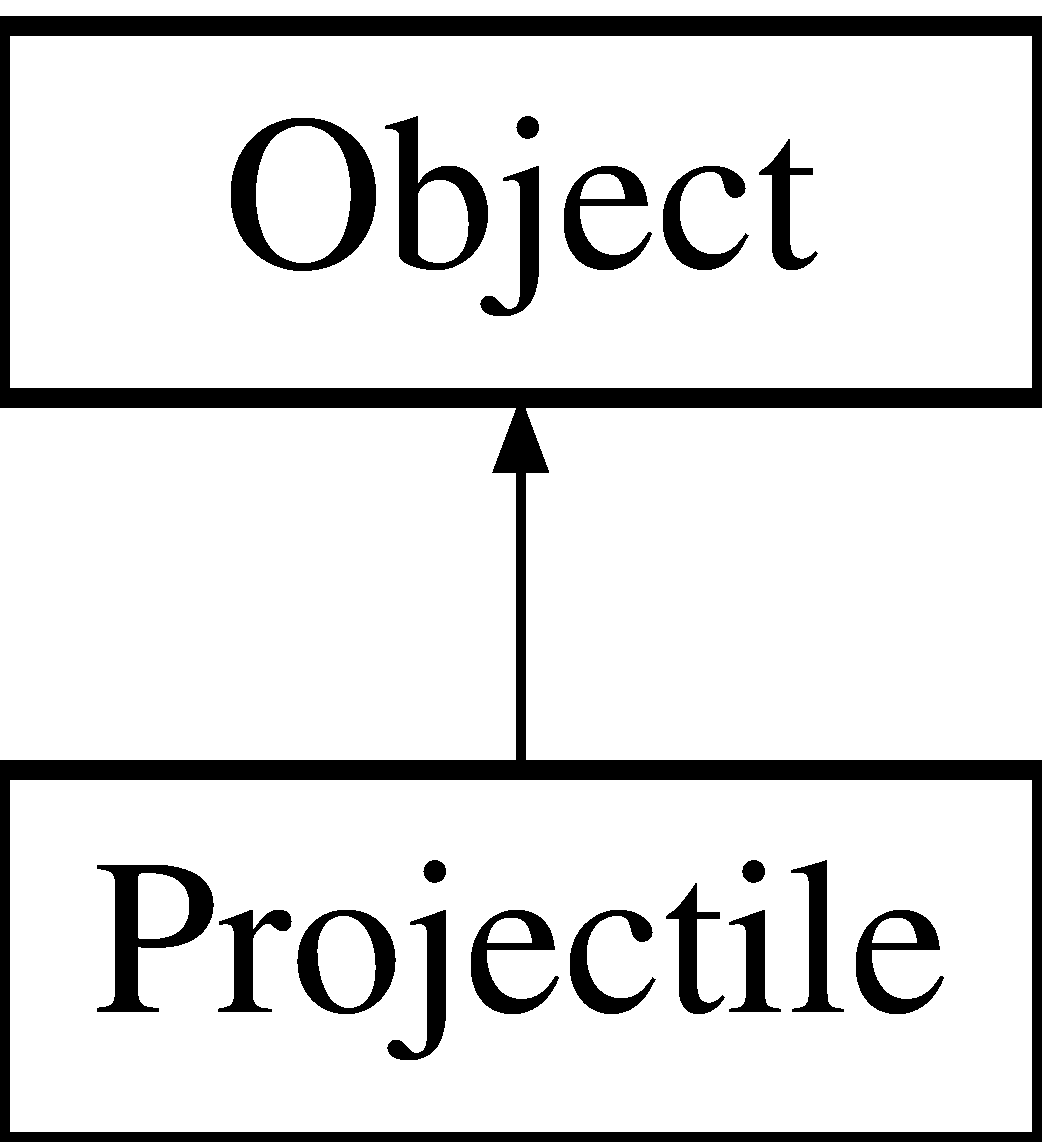
\includegraphics[height=2.000000cm]{classProjectile}
\end{center}
\end{figure}
\subsection*{Public Member Functions}
\begin{DoxyCompactItemize}
\item 
\hyperlink{classProjectile_a2ac17690fe70259fee93ec2d9be115d3}{Projectile} (Vector2d pos, Vector2d sp, double m, sf\+::\+Texture \&tex, std\+::shared\+\_\+ptr$<$ \hyperlink{classWorld}{World} $>$ w)
\item 
void \hyperlink{classProjectile_aa3781e4c9023c6d0306da7239987f9f7}{update\+State} (double dt)
\item 
void \hyperlink{classProjectile_abfd30c4ad89a47b267e269b9b6ab1300}{collide} (\hyperlink{classWall}{Wall} \&w)
\item 
virtual void \hyperlink{classProjectile_a5dbfa02e6e14a2149240762aa1e50403}{collide} (\hyperlink{classObject}{Object} \&o)
\item 
bool \hyperlink{classProjectile_abdb99a309b640e906790d93ad42511a4}{is\+Hit} ()
\item 
void \hyperlink{classProjectile_a6a409515a2e255b25ca80ee031d9a771}{set\+Hit} ()
\item 
bool \hyperlink{classProjectile_a02f748270bc39583e3268a88664f928e}{max\+Distance\+Surpassed} ()
\end{DoxyCompactItemize}
\subsection*{Additional Inherited Members}


\subsection{Detailed Description}
A class for the projectiles. 

\subsection{Constructor \& Destructor Documentation}
\hypertarget{classProjectile_a2ac17690fe70259fee93ec2d9be115d3}{}\label{classProjectile_a2ac17690fe70259fee93ec2d9be115d3} 
\index{Projectile@{Projectile}!Projectile@{Projectile}}
\index{Projectile@{Projectile}!Projectile@{Projectile}}
\subsubsection{\texorpdfstring{Projectile()}{Projectile()}}
{\footnotesize\ttfamily Projectile\+::\+Projectile (\begin{DoxyParamCaption}\item[{Vector2d}]{pos,  }\item[{Vector2d}]{sp,  }\item[{double}]{m,  }\item[{sf\+::\+Texture \&}]{tex,  }\item[{std\+::shared\+\_\+ptr$<$ \hyperlink{classWorld}{World} $>$}]{w }\end{DoxyParamCaption})}

Constructor 

\subsection{Member Function Documentation}
\hypertarget{classProjectile_abfd30c4ad89a47b267e269b9b6ab1300}{}\label{classProjectile_abfd30c4ad89a47b267e269b9b6ab1300} 
\index{Projectile@{Projectile}!collide@{collide}}
\index{collide@{collide}!Projectile@{Projectile}}
\subsubsection{\texorpdfstring{collide()}{collide()}\hspace{0.1cm}{\footnotesize\ttfamily [1/2]}}
{\footnotesize\ttfamily void Projectile\+::collide (\begin{DoxyParamCaption}\item[{\hyperlink{classWall}{Wall} \&}]{w }\end{DoxyParamCaption})}

Collides the projectile with a wall. \hypertarget{classProjectile_a5dbfa02e6e14a2149240762aa1e50403}{}\label{classProjectile_a5dbfa02e6e14a2149240762aa1e50403} 
\index{Projectile@{Projectile}!collide@{collide}}
\index{collide@{collide}!Projectile@{Projectile}}
\subsubsection{\texorpdfstring{collide()}{collide()}\hspace{0.1cm}{\footnotesize\ttfamily [2/2]}}
{\footnotesize\ttfamily void Projectile\+::collide (\begin{DoxyParamCaption}\item[{\hyperlink{classObject}{Object} \&}]{o }\end{DoxyParamCaption})\hspace{0.3cm}{\ttfamily [virtual]}}

Collides the projectile with an object. 

Implements \hyperlink{classObject}{Object}.

\hypertarget{classProjectile_abdb99a309b640e906790d93ad42511a4}{}\label{classProjectile_abdb99a309b640e906790d93ad42511a4} 
\index{Projectile@{Projectile}!is\+Hit@{is\+Hit}}
\index{is\+Hit@{is\+Hit}!Projectile@{Projectile}}
\subsubsection{\texorpdfstring{is\+Hit()}{isHit()}}
{\footnotesize\ttfamily bool Projectile\+::is\+Hit (\begin{DoxyParamCaption}{ }\end{DoxyParamCaption})\hspace{0.3cm}{\ttfamily [inline]}}

Returns whether the object is hit or not. \hypertarget{classProjectile_a02f748270bc39583e3268a88664f928e}{}\label{classProjectile_a02f748270bc39583e3268a88664f928e} 
\index{Projectile@{Projectile}!max\+Distance\+Surpassed@{max\+Distance\+Surpassed}}
\index{max\+Distance\+Surpassed@{max\+Distance\+Surpassed}!Projectile@{Projectile}}
\subsubsection{\texorpdfstring{max\+Distance\+Surpassed()}{maxDistanceSurpassed()}}
{\footnotesize\ttfamily bool Projectile\+::max\+Distance\+Surpassed (\begin{DoxyParamCaption}{ }\end{DoxyParamCaption})}

Checks whether the projectile has traveled its maximum distance. \hypertarget{classProjectile_a6a409515a2e255b25ca80ee031d9a771}{}\label{classProjectile_a6a409515a2e255b25ca80ee031d9a771} 
\index{Projectile@{Projectile}!set\+Hit@{set\+Hit}}
\index{set\+Hit@{set\+Hit}!Projectile@{Projectile}}
\subsubsection{\texorpdfstring{set\+Hit()}{setHit()}}
{\footnotesize\ttfamily void Projectile\+::set\+Hit (\begin{DoxyParamCaption}{ }\end{DoxyParamCaption})\hspace{0.3cm}{\ttfamily [inline]}}

Sets the projectile as hit. \hypertarget{classProjectile_aa3781e4c9023c6d0306da7239987f9f7}{}\label{classProjectile_aa3781e4c9023c6d0306da7239987f9f7} 
\index{Projectile@{Projectile}!update\+State@{update\+State}}
\index{update\+State@{update\+State}!Projectile@{Projectile}}
\subsubsection{\texorpdfstring{update\+State()}{updateState()}}
{\footnotesize\ttfamily void Projectile\+::update\+State (\begin{DoxyParamCaption}\item[{double}]{dt }\end{DoxyParamCaption})}

Updates the state of the projectile, meaning both its position and sprite. 

The documentation for this class was generated from the following files\+:\begin{DoxyCompactItemize}
\item 
src/projectile.\+hpp\item 
src/projectile.\+cpp\end{DoxyCompactItemize}

\hypertarget{classScreenEnd}{}\section{Screen\+End Class Reference}
\label{classScreenEnd}\index{Screen\+End@{Screen\+End}}


{\ttfamily \#include $<$screen\+\_\+end.\+hpp$>$}

Inheritance diagram for Screen\+End\+:\begin{figure}[H]
\begin{center}
\leavevmode
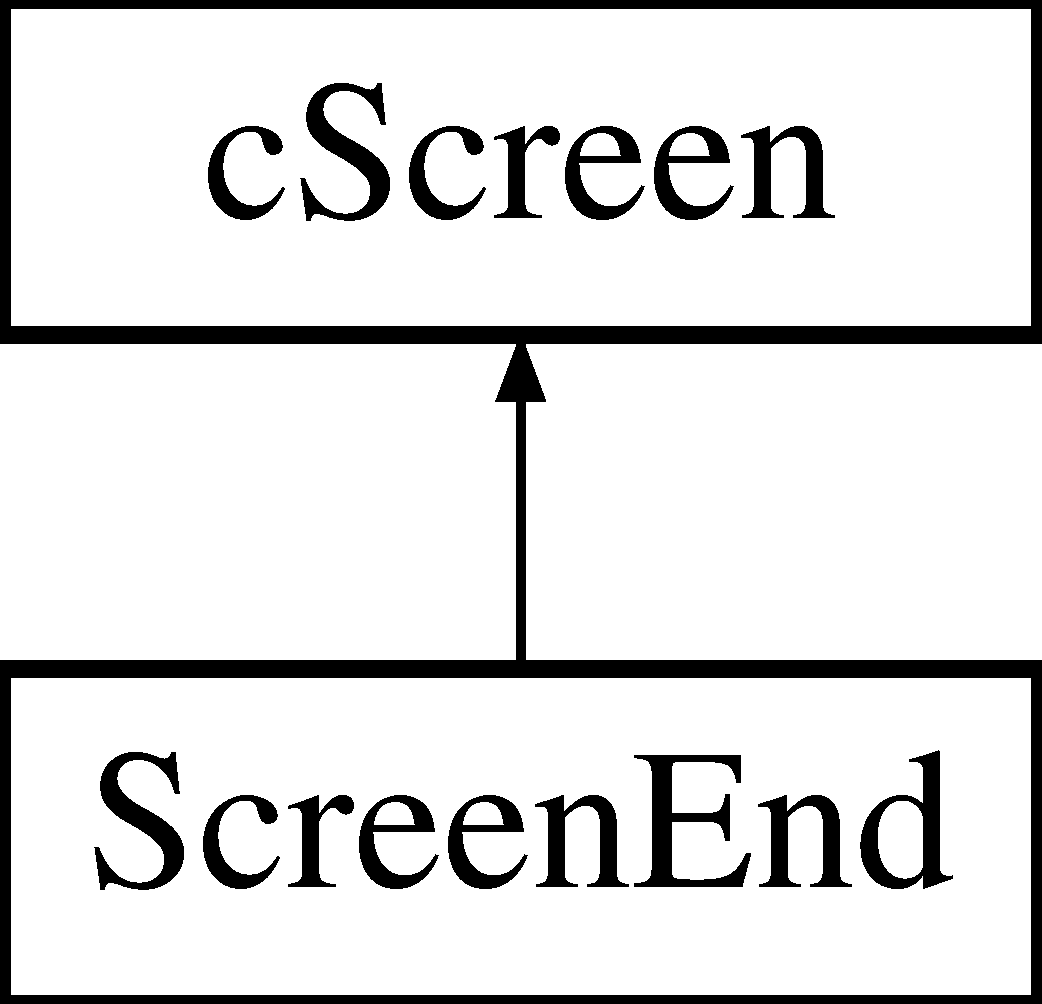
\includegraphics[height=2.000000cm]{classScreenEnd}
\end{center}
\end{figure}
\subsection*{Public Member Functions}
\begin{DoxyCompactItemize}
\item 
\hyperlink{classScreenEnd_a19ee749722201d3a47eb80729cdb176c}{Screen\+End} (std\+::shared\+\_\+ptr$<$ \hyperlink{classGameInfo}{Game\+Info} $>$ info)
\item 
int \hyperlink{classScreenEnd_a3582fcab70f5568fcdc187feeb1383ad}{Run} (sf\+::\+Render\+Window \&w)
\end{DoxyCompactItemize}


\subsection{Detailed Description}
End screen. 

\subsection{Constructor \& Destructor Documentation}
\hypertarget{classScreenEnd_a19ee749722201d3a47eb80729cdb176c}{}\label{classScreenEnd_a19ee749722201d3a47eb80729cdb176c} 
\index{Screen\+End@{Screen\+End}!Screen\+End@{Screen\+End}}
\index{Screen\+End@{Screen\+End}!Screen\+End@{Screen\+End}}
\subsubsection{\texorpdfstring{Screen\+End()}{ScreenEnd()}}
{\footnotesize\ttfamily Screen\+End\+::\+Screen\+End (\begin{DoxyParamCaption}\item[{std\+::shared\+\_\+ptr$<$ \hyperlink{classGameInfo}{Game\+Info} $>$}]{info }\end{DoxyParamCaption})\hspace{0.3cm}{\ttfamily [inline]}}

Constructor for end screen. 

\subsection{Member Function Documentation}
\hypertarget{classScreenEnd_a3582fcab70f5568fcdc187feeb1383ad}{}\label{classScreenEnd_a3582fcab70f5568fcdc187feeb1383ad} 
\index{Screen\+End@{Screen\+End}!Run@{Run}}
\index{Run@{Run}!Screen\+End@{Screen\+End}}
\subsubsection{\texorpdfstring{Run()}{Run()}}
{\footnotesize\ttfamily int Screen\+End\+::\+Run (\begin{DoxyParamCaption}\item[{sf\+::\+Render\+Window \&}]{w }\end{DoxyParamCaption})\hspace{0.3cm}{\ttfamily [virtual]}}

The actual end screen functionality. 

Implements \hyperlink{classcScreen_a4b4057ffec7ab1492a4de19f9994cac4}{c\+Screen}.



The documentation for this class was generated from the following files\+:\begin{DoxyCompactItemize}
\item 
src/screen\+\_\+end.\+hpp\item 
src/screen\+\_\+end.\+cpp\end{DoxyCompactItemize}

\hypertarget{classScreenInGame}{}\section{Screen\+In\+Game Class Reference}
\label{classScreenInGame}\index{Screen\+In\+Game@{Screen\+In\+Game}}


{\ttfamily \#include $<$screen\+\_\+ingame.\+hpp$>$}

Inheritance diagram for Screen\+In\+Game\+:\begin{figure}[H]
\begin{center}
\leavevmode
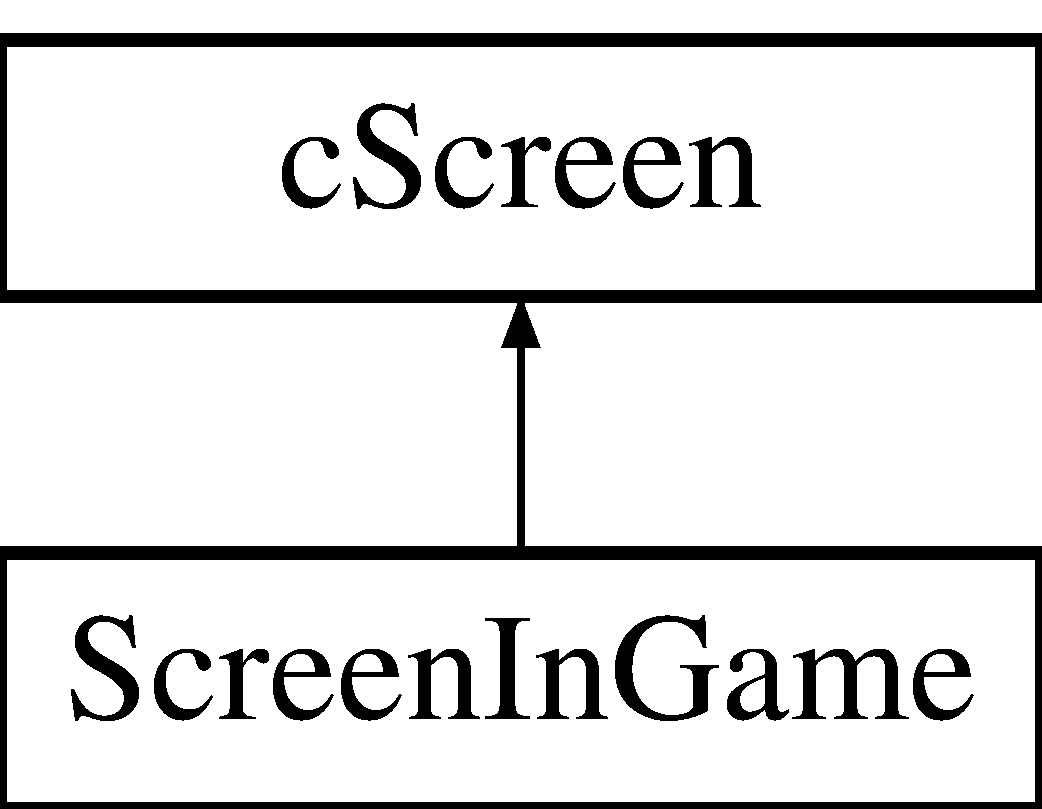
\includegraphics[height=2.000000cm]{classScreenInGame}
\end{center}
\end{figure}
\subsection*{Public Member Functions}
\begin{DoxyCompactItemize}
\item 
\hyperlink{classScreenInGame_aa2ce63e96970e0f19e589c61dcd914d0}{Screen\+In\+Game} (std\+::shared\+\_\+ptr$<$ \hyperlink{classGameInfo}{Game\+Info} $>$ info)
\item 
int \hyperlink{classScreenInGame_a55d4f45872f6d488145d1cf71819b960}{Run} (sf\+::\+Render\+Window \&)
\end{DoxyCompactItemize}


\subsection{Detailed Description}
Screen that contains the actual gameplay. Shares information with other sceens by using the \hyperlink{classGameInfo}{Game\+Info} class. 

\subsection{Constructor \& Destructor Documentation}
\hypertarget{classScreenInGame_aa2ce63e96970e0f19e589c61dcd914d0}{}\label{classScreenInGame_aa2ce63e96970e0f19e589c61dcd914d0} 
\index{Screen\+In\+Game@{Screen\+In\+Game}!Screen\+In\+Game@{Screen\+In\+Game}}
\index{Screen\+In\+Game@{Screen\+In\+Game}!Screen\+In\+Game@{Screen\+In\+Game}}
\subsubsection{\texorpdfstring{Screen\+In\+Game()}{ScreenInGame()}}
{\footnotesize\ttfamily Screen\+In\+Game\+::\+Screen\+In\+Game (\begin{DoxyParamCaption}\item[{std\+::shared\+\_\+ptr$<$ \hyperlink{classGameInfo}{Game\+Info} $>$}]{info }\end{DoxyParamCaption})\hspace{0.3cm}{\ttfamily [inline]}}

Constructor for the gameplay screen. 

\subsection{Member Function Documentation}
\hypertarget{classScreenInGame_a55d4f45872f6d488145d1cf71819b960}{}\label{classScreenInGame_a55d4f45872f6d488145d1cf71819b960} 
\index{Screen\+In\+Game@{Screen\+In\+Game}!Run@{Run}}
\index{Run@{Run}!Screen\+In\+Game@{Screen\+In\+Game}}
\subsubsection{\texorpdfstring{Run()}{Run()}}
{\footnotesize\ttfamily int Screen\+In\+Game\+::\+Run (\begin{DoxyParamCaption}\item[{sf\+::\+Render\+Window \&}]{w }\end{DoxyParamCaption})\hspace{0.3cm}{\ttfamily [virtual]}}

A function to run the scene. The actual gameplay or a menu is completely contained inside this function. 

Implements \hyperlink{classcScreen_a4b4057ffec7ab1492a4de19f9994cac4}{c\+Screen}.



The documentation for this class was generated from the following files\+:\begin{DoxyCompactItemize}
\item 
src/screen\+\_\+ingame.\+hpp\item 
src/screen\+\_\+ingame.\+cpp\end{DoxyCompactItemize}

\hypertarget{classScreenMenu}{}\section{Screen\+Menu Class Reference}
\label{classScreenMenu}\index{Screen\+Menu@{Screen\+Menu}}


{\ttfamily \#include $<$screen\+\_\+menu.\+hpp$>$}

Inheritance diagram for Screen\+Menu\+:\begin{figure}[H]
\begin{center}
\leavevmode
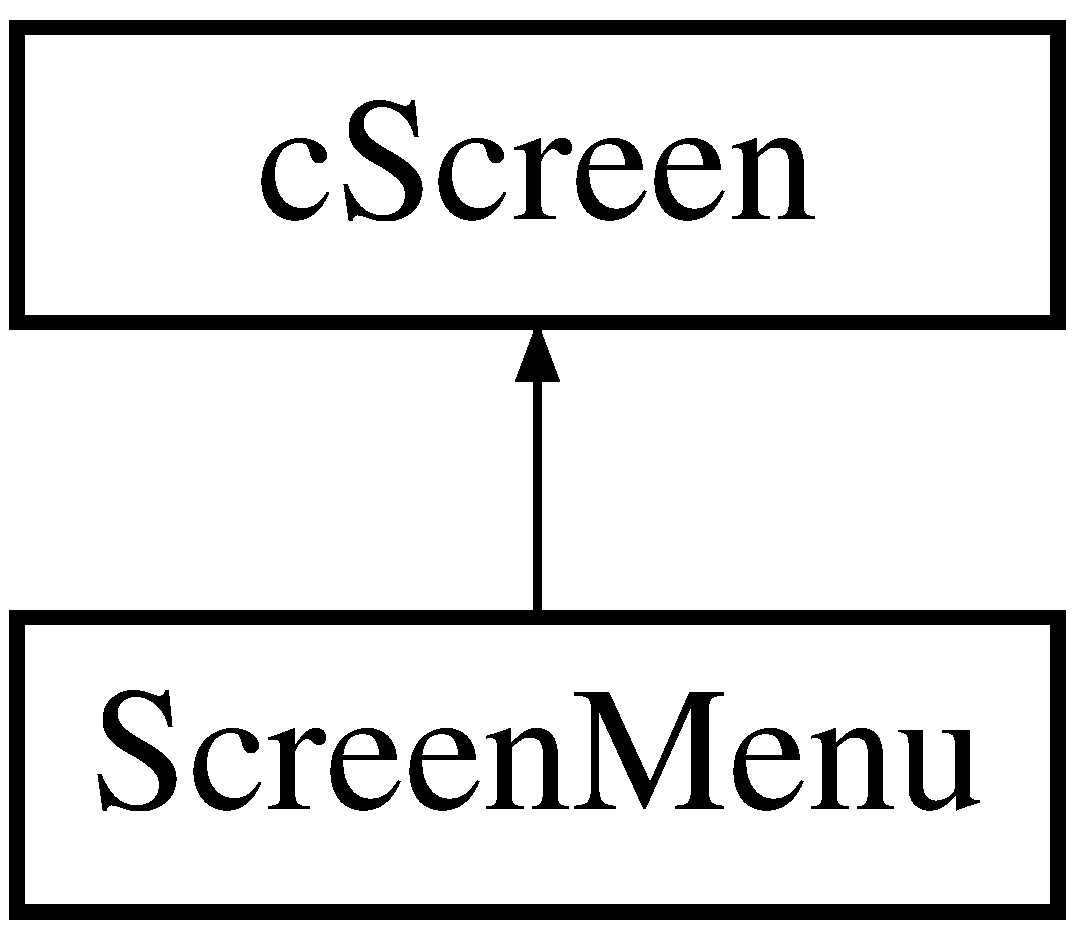
\includegraphics[height=2.000000cm]{classScreenMenu}
\end{center}
\end{figure}
\subsection*{Public Member Functions}
\begin{DoxyCompactItemize}
\item 
\hyperlink{classScreenMenu_a099466763f518ca39893224825c45968}{Screen\+Menu} (std\+::shared\+\_\+ptr$<$ \hyperlink{classGameInfo}{Game\+Info} $>$ info)
\item 
int \hyperlink{classScreenMenu_a86af8a6c97bf315bbe88cd2d7ab35abf}{Run} (sf\+::\+Render\+Window \&w)
\end{DoxyCompactItemize}


\subsection{Detailed Description}
Class dor the menu screen. 

\subsection{Constructor \& Destructor Documentation}
\hypertarget{classScreenMenu_a099466763f518ca39893224825c45968}{}\label{classScreenMenu_a099466763f518ca39893224825c45968} 
\index{Screen\+Menu@{Screen\+Menu}!Screen\+Menu@{Screen\+Menu}}
\index{Screen\+Menu@{Screen\+Menu}!Screen\+Menu@{Screen\+Menu}}
\subsubsection{\texorpdfstring{Screen\+Menu()}{ScreenMenu()}}
{\footnotesize\ttfamily Screen\+Menu\+::\+Screen\+Menu (\begin{DoxyParamCaption}\item[{std\+::shared\+\_\+ptr$<$ \hyperlink{classGameInfo}{Game\+Info} $>$}]{info }\end{DoxyParamCaption})\hspace{0.3cm}{\ttfamily [inline]}}

Constructor for the menu screen. 

\subsection{Member Function Documentation}
\hypertarget{classScreenMenu_a86af8a6c97bf315bbe88cd2d7ab35abf}{}\label{classScreenMenu_a86af8a6c97bf315bbe88cd2d7ab35abf} 
\index{Screen\+Menu@{Screen\+Menu}!Run@{Run}}
\index{Run@{Run}!Screen\+Menu@{Screen\+Menu}}
\subsubsection{\texorpdfstring{Run()}{Run()}}
{\footnotesize\ttfamily int Screen\+Menu\+::\+Run (\begin{DoxyParamCaption}\item[{sf\+::\+Render\+Window \&}]{w }\end{DoxyParamCaption})\hspace{0.3cm}{\ttfamily [virtual]}}

The actual menu screen functionality. 

Implements \hyperlink{classcScreen_a4b4057ffec7ab1492a4de19f9994cac4}{c\+Screen}.



The documentation for this class was generated from the following files\+:\begin{DoxyCompactItemize}
\item 
src/screen\+\_\+menu.\+hpp\item 
src/screen\+\_\+menu.\+cpp\end{DoxyCompactItemize}

\hypertarget{classTilemap}{}\section{Tilemap Class Reference}
\label{classTilemap}\index{Tilemap@{Tilemap}}


{\ttfamily \#include $<$tilemap.\+hpp$>$}

Inheritance diagram for Tilemap\+:\begin{figure}[H]
\begin{center}
\leavevmode
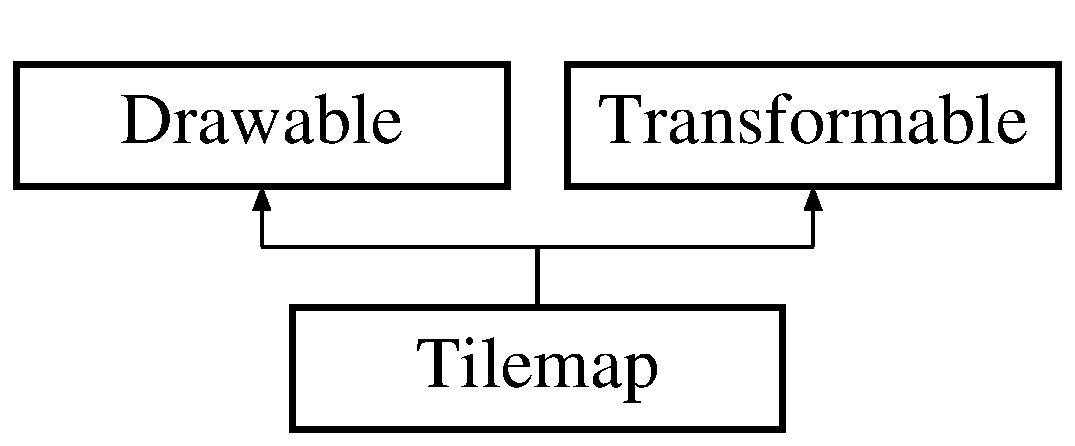
\includegraphics[height=2.000000cm]{classTilemap}
\end{center}
\end{figure}
\subsection*{Public Member Functions}
\begin{DoxyCompactItemize}
\item 
bool \hyperlink{classTilemap_a43d8cf3e3bd41fdf5215423d8fa4c846}{load} (std\+::string const \&tile\+Set\+Path, sf\+::\+Vector2u tilesize, Matrix map, int width, int height)
\end{DoxyCompactItemize}


\subsection{Detailed Description}
A class for the drawing of the game world map. \hyperlink{classTilemap}{Tilemap} contains the tiles that form the game map. This class is a slightly modified version of an example written by Laurent Gomila, licensed under the zlib/png license. 

\subsection{Member Function Documentation}
\hypertarget{classTilemap_a43d8cf3e3bd41fdf5215423d8fa4c846}{}\label{classTilemap_a43d8cf3e3bd41fdf5215423d8fa4c846} 
\index{Tilemap@{Tilemap}!load@{load}}
\index{load@{load}!Tilemap@{Tilemap}}
\subsubsection{\texorpdfstring{load()}{load()}}
{\footnotesize\ttfamily bool Tilemap\+::load (\begin{DoxyParamCaption}\item[{std\+::string const \&}]{tile\+Set\+Path,  }\item[{sf\+::\+Vector2u}]{tilesize,  }\item[{Matrix}]{map,  }\item[{int}]{width,  }\item[{int}]{height }\end{DoxyParamCaption})}

Creates the tilemap from a repserentation of the map as well as a tileset. 

The documentation for this class was generated from the following files\+:\begin{DoxyCompactItemize}
\item 
src/tilemap.\+hpp\item 
src/tilemap.\+cpp\end{DoxyCompactItemize}

\hypertarget{classVehicle}{}\section{Vehicle Class Reference}
\label{classVehicle}\index{Vehicle@{Vehicle}}


{\ttfamily \#include $<$vehicle.\+hpp$>$}

Inheritance diagram for Vehicle\+:\begin{figure}[H]
\begin{center}
\leavevmode
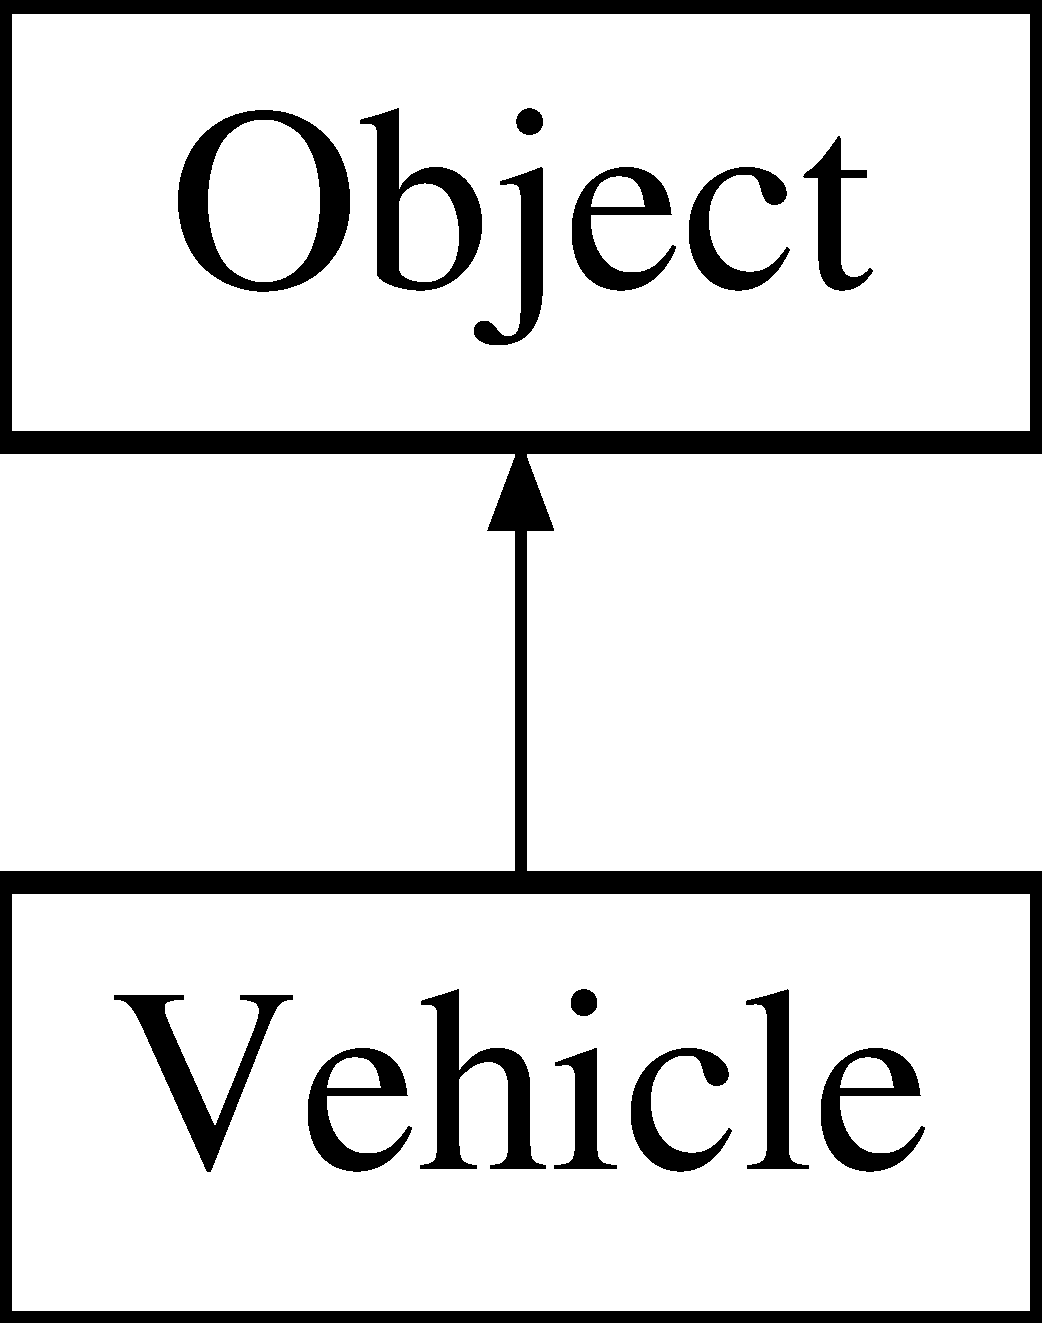
\includegraphics[height=2.000000cm]{classVehicle}
\end{center}
\end{figure}
\subsection*{Public Member Functions}
\begin{DoxyCompactItemize}
\item 
\hyperlink{classVehicle_a60b696997b412b5dd48728bbc3f56dce}{Vehicle} (Vector2d pos, double orientation\+Angle, double max\+Sp, double maxF, double m, std\+::shared\+\_\+ptr$<$ \hyperlink{classPlayerInput}{Player\+Input} $>$ p1, std\+::shared\+\_\+ptr$<$ \hyperlink{classWorld}{World} $>$ w)
\item 
void \hyperlink{classVehicle_af1ea3f326eb5ca27e1a06f4fe81832ce}{update\+State} (double dt)
\item 
virtual void \hyperlink{classVehicle_ab1fbef5c7898343380c1d9aaab11c64a}{set\+Texture} (std\+::string path)
\item 
void \hyperlink{classVehicle_adfc1996e318be79103e6d34eb60da656}{set\+Ammo\+Texture} (std\+::string path)
\item 
void \hyperlink{classVehicle_a54a02d80bb7693b7e9e2b00bd1ef3217}{shoot} (std\+::shared\+\_\+ptr$<$ \hyperlink{classWorld}{World} $>$ world)
\item 
int \hyperlink{classVehicle_aa3ec0152e6944dcd9e3b219dbf4fbba5}{get\+Lap} () const
\end{DoxyCompactItemize}
\subsection*{Additional Inherited Members}


\subsection{Detailed Description}
A class for containing the vehicles in the game. A vehicle is derived from the object class, and therefore has the physical properties that an object has. 

\subsection{Constructor \& Destructor Documentation}
\hypertarget{classVehicle_a60b696997b412b5dd48728bbc3f56dce}{}\label{classVehicle_a60b696997b412b5dd48728bbc3f56dce} 
\index{Vehicle@{Vehicle}!Vehicle@{Vehicle}}
\index{Vehicle@{Vehicle}!Vehicle@{Vehicle}}
\subsubsection{\texorpdfstring{Vehicle()}{Vehicle()}}
{\footnotesize\ttfamily Vehicle\+::\+Vehicle (\begin{DoxyParamCaption}\item[{Vector2d}]{pos,  }\item[{double}]{orientation\+Angle,  }\item[{double}]{max\+Sp,  }\item[{double}]{maxF,  }\item[{double}]{m,  }\item[{std\+::shared\+\_\+ptr$<$ \hyperlink{classPlayerInput}{Player\+Input} $>$}]{p1,  }\item[{std\+::shared\+\_\+ptr$<$ \hyperlink{classWorld}{World} $>$}]{w }\end{DoxyParamCaption})}

Constructor 

\subsection{Member Function Documentation}
\hypertarget{classVehicle_aa3ec0152e6944dcd9e3b219dbf4fbba5}{}\label{classVehicle_aa3ec0152e6944dcd9e3b219dbf4fbba5} 
\index{Vehicle@{Vehicle}!get\+Lap@{get\+Lap}}
\index{get\+Lap@{get\+Lap}!Vehicle@{Vehicle}}
\subsubsection{\texorpdfstring{get\+Lap()}{getLap()}}
{\footnotesize\ttfamily int Vehicle\+::get\+Lap (\begin{DoxyParamCaption}{ }\end{DoxyParamCaption}) const\hspace{0.3cm}{\ttfamily [inline]}}

Returns the lap the vehicle is currently on. \hypertarget{classVehicle_adfc1996e318be79103e6d34eb60da656}{}\label{classVehicle_adfc1996e318be79103e6d34eb60da656} 
\index{Vehicle@{Vehicle}!set\+Ammo\+Texture@{set\+Ammo\+Texture}}
\index{set\+Ammo\+Texture@{set\+Ammo\+Texture}!Vehicle@{Vehicle}}
\subsubsection{\texorpdfstring{set\+Ammo\+Texture()}{setAmmoTexture()}}
{\footnotesize\ttfamily void Vehicle\+::set\+Ammo\+Texture (\begin{DoxyParamCaption}\item[{std\+::string}]{path }\end{DoxyParamCaption})}

Sets a texture for the ammo type the vehicle uses. \hypertarget{classVehicle_ab1fbef5c7898343380c1d9aaab11c64a}{}\label{classVehicle_ab1fbef5c7898343380c1d9aaab11c64a} 
\index{Vehicle@{Vehicle}!set\+Texture@{set\+Texture}}
\index{set\+Texture@{set\+Texture}!Vehicle@{Vehicle}}
\subsubsection{\texorpdfstring{set\+Texture()}{setTexture()}}
{\footnotesize\ttfamily void Vehicle\+::set\+Texture (\begin{DoxyParamCaption}\item[{std\+::string}]{path }\end{DoxyParamCaption})\hspace{0.3cm}{\ttfamily [virtual]}}

Sets the texture for the vehicle. \hypertarget{classVehicle_a54a02d80bb7693b7e9e2b00bd1ef3217}{}\label{classVehicle_a54a02d80bb7693b7e9e2b00bd1ef3217} 
\index{Vehicle@{Vehicle}!shoot@{shoot}}
\index{shoot@{shoot}!Vehicle@{Vehicle}}
\subsubsection{\texorpdfstring{shoot()}{shoot()}}
{\footnotesize\ttfamily void Vehicle\+::shoot (\begin{DoxyParamCaption}\item[{std\+::shared\+\_\+ptr$<$ \hyperlink{classWorld}{World} $>$}]{world }\end{DoxyParamCaption})}

This function handles the shooting of a projectile. \hypertarget{classVehicle_af1ea3f326eb5ca27e1a06f4fe81832ce}{}\label{classVehicle_af1ea3f326eb5ca27e1a06f4fe81832ce} 
\index{Vehicle@{Vehicle}!update\+State@{update\+State}}
\index{update\+State@{update\+State}!Vehicle@{Vehicle}}
\subsubsection{\texorpdfstring{update\+State()}{updateState()}}
{\footnotesize\ttfamily void Vehicle\+::update\+State (\begin{DoxyParamCaption}\item[{double}]{dt }\end{DoxyParamCaption})}

Updates the state of the vehicle. This includes both the physics as well as the input for the vehicle. 

The documentation for this class was generated from the following files\+:\begin{DoxyCompactItemize}
\item 
src/vehicle.\+hpp\item 
src/vehicle.\+cpp\end{DoxyCompactItemize}

\hypertarget{structVehicleInfo}{}\section{Vehicle\+Info Struct Reference}
\label{structVehicleInfo}\index{Vehicle\+Info@{Vehicle\+Info}}


{\ttfamily \#include $<$vehicle.\+hpp$>$}

\subsection*{Public Attributes}
\begin{DoxyCompactItemize}
\item 
\hypertarget{structVehicleInfo_ab9d63eb653459385a027ee308e995ed4}{}\label{structVehicleInfo_ab9d63eb653459385a027ee308e995ed4} 
Vector2d {\bfseries position1}
\item 
\hypertarget{structVehicleInfo_a2ff369facb2f93ee770bdedad85fd734}{}\label{structVehicleInfo_a2ff369facb2f93ee770bdedad85fd734} 
Vector2d {\bfseries position2}
\item 
\hypertarget{structVehicleInfo_a0ed3789a6f9a444395bd23bc13793e0a}{}\label{structVehicleInfo_a0ed3789a6f9a444395bd23bc13793e0a} 
double {\bfseries orientation}
\item 
\hypertarget{structVehicleInfo_aa9161f00b5082bdc903cdfbf708ee7cb}{}\label{structVehicleInfo_aa9161f00b5082bdc903cdfbf708ee7cb} 
double {\bfseries max\+Sp}
\item 
\hypertarget{structVehicleInfo_a0f1cb051100bbd38c0e5e99dfb3dd149}{}\label{structVehicleInfo_a0f1cb051100bbd38c0e5e99dfb3dd149} 
double {\bfseries maxF}
\item 
\hypertarget{structVehicleInfo_a56d7d3b9a791542e3765303e0007e2fc}{}\label{structVehicleInfo_a56d7d3b9a791542e3765303e0007e2fc} 
double {\bfseries mass}
\end{DoxyCompactItemize}


\subsection{Detailed Description}
A structure for setting the initial configurations for vehicles in a map. 

The documentation for this struct was generated from the following file\+:\begin{DoxyCompactItemize}
\item 
src/vehicle.\+hpp\end{DoxyCompactItemize}

\hypertarget{classWall}{}\section{Wall Class Reference}
\label{classWall}\index{Wall@{Wall}}


{\ttfamily \#include $<$wall.\+hpp$>$}

Inheritance diagram for Wall\+:\begin{figure}[H]
\begin{center}
\leavevmode
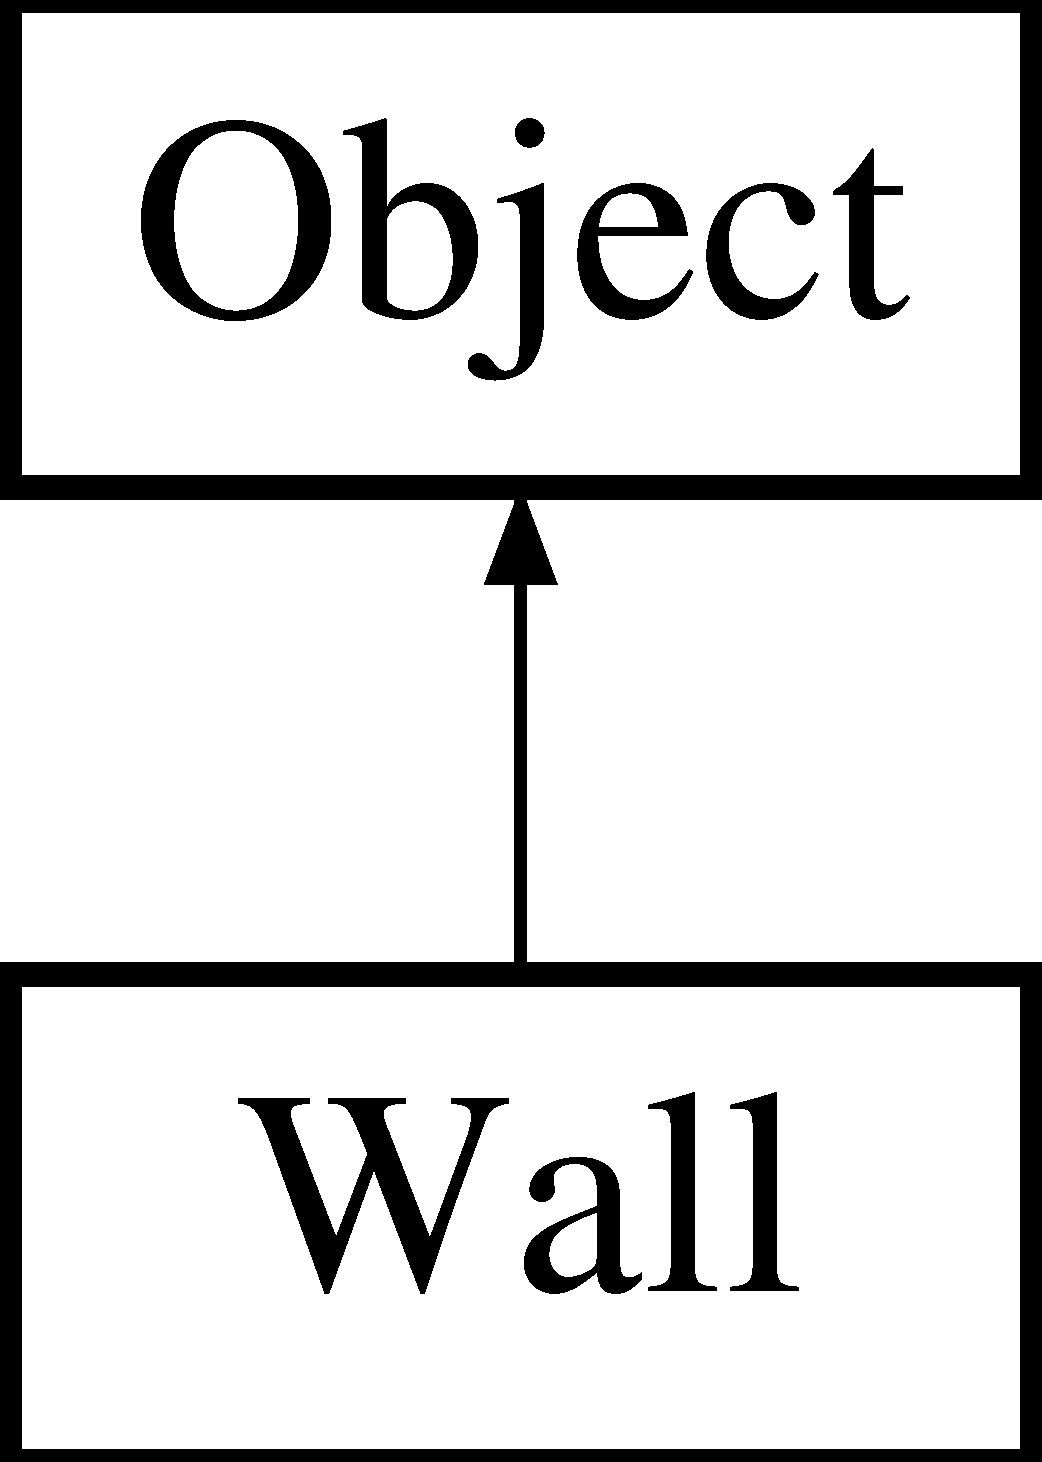
\includegraphics[height=2.000000cm]{classWall}
\end{center}
\end{figure}
\subsection*{Public Member Functions}
\begin{DoxyCompactItemize}
\item 
\hyperlink{classWall_a769393b378fa304cfe1f1c10e9283514}{Wall} (Vector2d pos, int w, int h, double orientation\+Angle=0)
\item 
void \hyperlink{classWall_aae68a37386f56e928ccdbd55c4464550}{collide} (\hyperlink{classObject}{Object} \&o)
\item 
const double \& \hyperlink{classWall_a98f9c3ef8a89ee2622e1cf84df093a2d}{get\+Width} () const
\item 
const double \& \hyperlink{classWall_a9be8bb3c3696aeaf01b3d9dfaf9462cf}{get\+Height} () const
\end{DoxyCompactItemize}
\subsection*{Additional Inherited Members}


\subsection{Detailed Description}
A class for the walls in our game world. 

\subsection{Constructor \& Destructor Documentation}
\hypertarget{classWall_a769393b378fa304cfe1f1c10e9283514}{}\label{classWall_a769393b378fa304cfe1f1c10e9283514} 
\index{Wall@{Wall}!Wall@{Wall}}
\index{Wall@{Wall}!Wall@{Wall}}
\subsubsection{\texorpdfstring{Wall()}{Wall()}}
{\footnotesize\ttfamily Wall\+::\+Wall (\begin{DoxyParamCaption}\item[{Vector2d}]{pos,  }\item[{int}]{w,  }\item[{int}]{h,  }\item[{double}]{orientation\+Angle = {\ttfamily 0} }\end{DoxyParamCaption})\hspace{0.3cm}{\ttfamily [inline]}}

Constructor 

\subsection{Member Function Documentation}
\hypertarget{classWall_aae68a37386f56e928ccdbd55c4464550}{}\label{classWall_aae68a37386f56e928ccdbd55c4464550} 
\index{Wall@{Wall}!collide@{collide}}
\index{collide@{collide}!Wall@{Wall}}
\subsubsection{\texorpdfstring{collide()}{collide()}}
{\footnotesize\ttfamily void Wall\+::collide (\begin{DoxyParamCaption}\item[{\hyperlink{classObject}{Object} \&}]{o }\end{DoxyParamCaption})\hspace{0.3cm}{\ttfamily [virtual]}}

A function for colliding with objects. 

Implements \hyperlink{classObject}{Object}.

\hypertarget{classWall_a9be8bb3c3696aeaf01b3d9dfaf9462cf}{}\label{classWall_a9be8bb3c3696aeaf01b3d9dfaf9462cf} 
\index{Wall@{Wall}!get\+Height@{get\+Height}}
\index{get\+Height@{get\+Height}!Wall@{Wall}}
\subsubsection{\texorpdfstring{get\+Height()}{getHeight()}}
{\footnotesize\ttfamily const double \& Wall\+::get\+Height (\begin{DoxyParamCaption}{ }\end{DoxyParamCaption}) const}

Returns the height of the wall. \hypertarget{classWall_a98f9c3ef8a89ee2622e1cf84df093a2d}{}\label{classWall_a98f9c3ef8a89ee2622e1cf84df093a2d} 
\index{Wall@{Wall}!get\+Width@{get\+Width}}
\index{get\+Width@{get\+Width}!Wall@{Wall}}
\subsubsection{\texorpdfstring{get\+Width()}{getWidth()}}
{\footnotesize\ttfamily const double \& Wall\+::get\+Width (\begin{DoxyParamCaption}{ }\end{DoxyParamCaption}) const}

Returns the width of the wall 

The documentation for this class was generated from the following files\+:\begin{DoxyCompactItemize}
\item 
src/wall.\+hpp\item 
src/wall.\+cpp\end{DoxyCompactItemize}

\hypertarget{classWorld}{}\section{World Class Reference}
\label{classWorld}\index{World@{World}}


{\ttfamily \#include $<$world.\+hpp$>$}

\subsection*{Public Member Functions}
\begin{DoxyCompactItemize}
\item 
void \hyperlink{classWorld_a5160225e83eae7837e624ef90d4db29f}{add\+Vehicle} (Vehicle\+Ptr v)
\item 
void \hyperlink{classWorld_a0dabad321c25115c1899d53b0525f1ff}{add\+Projectile} (Projectile\+Ptr p)
\item 
void \hyperlink{classWorld_aee0ecea7671c2b87896ae48e2b8b4db0}{add\+Wall} (Wall\+Ptr w)
\item 
void \hyperlink{classWorld_ae732dc0bbb384d5799c17b18f20ff52d}{add\+Check\+Points} (std\+::vector$<$ Cp\+Ptr $>$ c)
\item 
void \hyperlink{classWorld_a6cfa1ac0ab2d191cddb6273119b2e8b6}{add\+Mines} (std\+::vector$<$ Mine\+Ptr $>$ m)
\item 
void \hyperlink{classWorld_afbde7c41f335e5abdf67935e4ef39d12}{add\+Map} (Map\+Ptr m)
\item 
void \hyperlink{classWorld_a0fa5babafd1bb5749f7f3d664cf996c5}{add\+Vehicle\+Info} (std\+::shared\+\_\+ptr$<$ \hyperlink{structVehicleInfo}{Vehicle\+Info} $>$)
\item 
std\+::vector$<$ Vehicle\+Ptr $>$ \hyperlink{classWorld_afa144f2f17a04087776721af7b225387}{get\+Vehicles} () const
\item 
std\+::vector$<$ Projectile\+Ptr $>$ \hyperlink{classWorld_a52e57fb3229773869172a71d49b29783}{get\+Projectiles} () const
\item 
Map\+Ptr \hyperlink{classWorld_a37b996591688a176897dc8157cdbb18d}{get\+Map} () const
\item 
std\+::shared\+\_\+ptr$<$ \hyperlink{structVehicleInfo}{Vehicle\+Info} $>$ \hyperlink{classWorld_a74d8300035e9495d954e5f6ef90b64b5}{get\+Vehicle\+Info} () const
\item 
std\+::vector$<$ Wall\+Ptr $>$ \hyperlink{classWorld_a2abd0169432b982782a77914bffd3fa0}{get\+Walls} () const
\item 
std\+::vector$<$ Cp\+Ptr $>$ \hyperlink{classWorld_a86ec41dd36a293bd86f6ed9070863c19}{get\+Check\+Points} () const
\item 
std\+::vector$<$ Mine\+Ptr $>$ \hyperlink{classWorld_a0003fd04b63a37ae393879083f2db673}{get\+Mines} () const
\item 
int \hyperlink{classWorld_a976371693de928677ae490df24519696}{get\+Lap\+Total} () const
\item 
std\+::vector$<$ sf\+::\+View $>$ \hyperlink{classWorld_acc906e59c83bbed0da781ae9e4981d4c}{set\+Views} (Window \&w) const
\item 
void \hyperlink{classWorld_a1958eb9641efaa29bff034f4e076f10a}{set\+Font} (std\+::shared\+\_\+ptr$<$ sf\+::\+Font $>$ f)
\item 
void \hyperlink{classWorld_aea52953b00dfbea7766176454206b007}{update\+State} (double dt)
\item 
void \hyperlink{classWorld_acf70b954c41a9c086d8678da4b95a9a4}{draw} (Window \&w)
\end{DoxyCompactItemize}


\subsection{Detailed Description}
A class that contains the game world and everything in it. Is responsible for updating the game logic as well as drawing the game world. 

\subsection{Member Function Documentation}
\hypertarget{classWorld_ae732dc0bbb384d5799c17b18f20ff52d}{}\label{classWorld_ae732dc0bbb384d5799c17b18f20ff52d} 
\index{World@{World}!add\+Check\+Points@{add\+Check\+Points}}
\index{add\+Check\+Points@{add\+Check\+Points}!World@{World}}
\subsubsection{\texorpdfstring{add\+Check\+Points()}{addCheckPoints()}}
{\footnotesize\ttfamily void World\+::add\+Check\+Points (\begin{DoxyParamCaption}\item[{std\+::vector$<$ Cp\+Ptr $>$}]{c }\end{DoxyParamCaption})}

Adds the map checkpoints to world. \hypertarget{classWorld_afbde7c41f335e5abdf67935e4ef39d12}{}\label{classWorld_afbde7c41f335e5abdf67935e4ef39d12} 
\index{World@{World}!add\+Map@{add\+Map}}
\index{add\+Map@{add\+Map}!World@{World}}
\subsubsection{\texorpdfstring{add\+Map()}{addMap()}}
{\footnotesize\ttfamily void World\+::add\+Map (\begin{DoxyParamCaption}\item[{Map\+Ptr}]{m }\end{DoxyParamCaption})}

Adds the game map to world. \hypertarget{classWorld_a6cfa1ac0ab2d191cddb6273119b2e8b6}{}\label{classWorld_a6cfa1ac0ab2d191cddb6273119b2e8b6} 
\index{World@{World}!add\+Mines@{add\+Mines}}
\index{add\+Mines@{add\+Mines}!World@{World}}
\subsubsection{\texorpdfstring{add\+Mines()}{addMines()}}
{\footnotesize\ttfamily void World\+::add\+Mines (\begin{DoxyParamCaption}\item[{std\+::vector$<$ Mine\+Ptr $>$}]{m }\end{DoxyParamCaption})}

Adds mines to world. \hypertarget{classWorld_a0dabad321c25115c1899d53b0525f1ff}{}\label{classWorld_a0dabad321c25115c1899d53b0525f1ff} 
\index{World@{World}!add\+Projectile@{add\+Projectile}}
\index{add\+Projectile@{add\+Projectile}!World@{World}}
\subsubsection{\texorpdfstring{add\+Projectile()}{addProjectile()}}
{\footnotesize\ttfamily void World\+::add\+Projectile (\begin{DoxyParamCaption}\item[{Projectile\+Ptr}]{p }\end{DoxyParamCaption})}

Adds a projectile smart pointer to world. \hypertarget{classWorld_a5160225e83eae7837e624ef90d4db29f}{}\label{classWorld_a5160225e83eae7837e624ef90d4db29f} 
\index{World@{World}!add\+Vehicle@{add\+Vehicle}}
\index{add\+Vehicle@{add\+Vehicle}!World@{World}}
\subsubsection{\texorpdfstring{add\+Vehicle()}{addVehicle()}}
{\footnotesize\ttfamily void World\+::add\+Vehicle (\begin{DoxyParamCaption}\item[{Vehicle\+Ptr}]{v }\end{DoxyParamCaption})}

Adds a vehicle smart pointer to world. \hypertarget{classWorld_a0fa5babafd1bb5749f7f3d664cf996c5}{}\label{classWorld_a0fa5babafd1bb5749f7f3d664cf996c5} 
\index{World@{World}!add\+Vehicle\+Info@{add\+Vehicle\+Info}}
\index{add\+Vehicle\+Info@{add\+Vehicle\+Info}!World@{World}}
\subsubsection{\texorpdfstring{add\+Vehicle\+Info()}{addVehicleInfo()}}
{\footnotesize\ttfamily void World\+::add\+Vehicle\+Info (\begin{DoxyParamCaption}\item[{std\+::shared\+\_\+ptr$<$ \hyperlink{structVehicleInfo}{Vehicle\+Info} $>$}]{ }\end{DoxyParamCaption})}

Reads vehicle info from maps \hypertarget{classWorld_aee0ecea7671c2b87896ae48e2b8b4db0}{}\label{classWorld_aee0ecea7671c2b87896ae48e2b8b4db0} 
\index{World@{World}!add\+Wall@{add\+Wall}}
\index{add\+Wall@{add\+Wall}!World@{World}}
\subsubsection{\texorpdfstring{add\+Wall()}{addWall()}}
{\footnotesize\ttfamily void World\+::add\+Wall (\begin{DoxyParamCaption}\item[{Wall\+Ptr}]{w }\end{DoxyParamCaption})}

Adds a wall smart pointer to world. \hypertarget{classWorld_acf70b954c41a9c086d8678da4b95a9a4}{}\label{classWorld_acf70b954c41a9c086d8678da4b95a9a4} 
\index{World@{World}!draw@{draw}}
\index{draw@{draw}!World@{World}}
\subsubsection{\texorpdfstring{draw()}{draw()}}
{\footnotesize\ttfamily void World\+::draw (\begin{DoxyParamCaption}\item[{Window \&}]{w }\end{DoxyParamCaption})}

Draws the game world to a window. \hypertarget{classWorld_a86ec41dd36a293bd86f6ed9070863c19}{}\label{classWorld_a86ec41dd36a293bd86f6ed9070863c19} 
\index{World@{World}!get\+Check\+Points@{get\+Check\+Points}}
\index{get\+Check\+Points@{get\+Check\+Points}!World@{World}}
\subsubsection{\texorpdfstring{get\+Check\+Points()}{getCheckPoints()}}
{\footnotesize\ttfamily std\+::vector$<$ std\+::shared\+\_\+ptr$<$ \hyperlink{classCheckPoint}{Check\+Point} $>$ $>$ World\+::get\+Check\+Points (\begin{DoxyParamCaption}{ }\end{DoxyParamCaption}) const}

gets the map checkpoints. \hypertarget{classWorld_a976371693de928677ae490df24519696}{}\label{classWorld_a976371693de928677ae490df24519696} 
\index{World@{World}!get\+Lap\+Total@{get\+Lap\+Total}}
\index{get\+Lap\+Total@{get\+Lap\+Total}!World@{World}}
\subsubsection{\texorpdfstring{get\+Lap\+Total()}{getLapTotal()}}
{\footnotesize\ttfamily int World\+::get\+Lap\+Total (\begin{DoxyParamCaption}{ }\end{DoxyParamCaption}) const\hspace{0.3cm}{\ttfamily [inline]}}

Returns the total amount of laps in the race. \hypertarget{classWorld_a37b996591688a176897dc8157cdbb18d}{}\label{classWorld_a37b996591688a176897dc8157cdbb18d} 
\index{World@{World}!get\+Map@{get\+Map}}
\index{get\+Map@{get\+Map}!World@{World}}
\subsubsection{\texorpdfstring{get\+Map()}{getMap()}}
{\footnotesize\ttfamily Map\+Ptr World\+::get\+Map (\begin{DoxyParamCaption}{ }\end{DoxyParamCaption}) const}

Returns the game map \hypertarget{classWorld_a0003fd04b63a37ae393879083f2db673}{}\label{classWorld_a0003fd04b63a37ae393879083f2db673} 
\index{World@{World}!get\+Mines@{get\+Mines}}
\index{get\+Mines@{get\+Mines}!World@{World}}
\subsubsection{\texorpdfstring{get\+Mines()}{getMines()}}
{\footnotesize\ttfamily std\+::vector$<$ std\+::shared\+\_\+ptr$<$ \hyperlink{classMine}{Mine} $>$ $>$ World\+::get\+Mines (\begin{DoxyParamCaption}{ }\end{DoxyParamCaption}) const}

Gets a list of mines from world. \hypertarget{classWorld_a52e57fb3229773869172a71d49b29783}{}\label{classWorld_a52e57fb3229773869172a71d49b29783} 
\index{World@{World}!get\+Projectiles@{get\+Projectiles}}
\index{get\+Projectiles@{get\+Projectiles}!World@{World}}
\subsubsection{\texorpdfstring{get\+Projectiles()}{getProjectiles()}}
{\footnotesize\ttfamily std\+::vector$<$ Projectile\+Ptr $>$ World\+::get\+Projectiles (\begin{DoxyParamCaption}{ }\end{DoxyParamCaption}) const}

A method to get the projectiles inside the world \hypertarget{classWorld_a74d8300035e9495d954e5f6ef90b64b5}{}\label{classWorld_a74d8300035e9495d954e5f6ef90b64b5} 
\index{World@{World}!get\+Vehicle\+Info@{get\+Vehicle\+Info}}
\index{get\+Vehicle\+Info@{get\+Vehicle\+Info}!World@{World}}
\subsubsection{\texorpdfstring{get\+Vehicle\+Info()}{getVehicleInfo()}}
{\footnotesize\ttfamily std\+::shared\+\_\+ptr$<$ \hyperlink{structVehicleInfo}{Vehicle\+Info} $>$ World\+::get\+Vehicle\+Info (\begin{DoxyParamCaption}{ }\end{DoxyParamCaption}) const}

A Method to fetch vehicle info from world. \hypertarget{classWorld_afa144f2f17a04087776721af7b225387}{}\label{classWorld_afa144f2f17a04087776721af7b225387} 
\index{World@{World}!get\+Vehicles@{get\+Vehicles}}
\index{get\+Vehicles@{get\+Vehicles}!World@{World}}
\subsubsection{\texorpdfstring{get\+Vehicles()}{getVehicles()}}
{\footnotesize\ttfamily std\+::vector$<$ Vehicle\+Ptr $>$ World\+::get\+Vehicles (\begin{DoxyParamCaption}{ }\end{DoxyParamCaption}) const}

A method to get the vehicles inside the world \hypertarget{classWorld_a2abd0169432b982782a77914bffd3fa0}{}\label{classWorld_a2abd0169432b982782a77914bffd3fa0} 
\index{World@{World}!get\+Walls@{get\+Walls}}
\index{get\+Walls@{get\+Walls}!World@{World}}
\subsubsection{\texorpdfstring{get\+Walls()}{getWalls()}}
{\footnotesize\ttfamily std\+::vector$<$ Wall\+Ptr $>$ World\+::get\+Walls (\begin{DoxyParamCaption}{ }\end{DoxyParamCaption}) const}

gets the walls from world. \hypertarget{classWorld_a1958eb9641efaa29bff034f4e076f10a}{}\label{classWorld_a1958eb9641efaa29bff034f4e076f10a} 
\index{World@{World}!set\+Font@{set\+Font}}
\index{set\+Font@{set\+Font}!World@{World}}
\subsubsection{\texorpdfstring{set\+Font()}{setFont()}}
{\footnotesize\ttfamily void World\+::set\+Font (\begin{DoxyParamCaption}\item[{std\+::shared\+\_\+ptr$<$ sf\+::\+Font $>$}]{f }\end{DoxyParamCaption})}

Sets a font for world. \hypertarget{classWorld_acc906e59c83bbed0da781ae9e4981d4c}{}\label{classWorld_acc906e59c83bbed0da781ae9e4981d4c} 
\index{World@{World}!set\+Views@{set\+Views}}
\index{set\+Views@{set\+Views}!World@{World}}
\subsubsection{\texorpdfstring{set\+Views()}{setViews()}}
{\footnotesize\ttfamily std\+::vector$<$ sf\+::\+View $>$ World\+::set\+Views (\begin{DoxyParamCaption}\item[{Window \&}]{w }\end{DoxyParamCaption}) const}

Sets the split-\/screen view necessary for 2-\/player play and returns a list of the views. \hypertarget{classWorld_aea52953b00dfbea7766176454206b007}{}\label{classWorld_aea52953b00dfbea7766176454206b007} 
\index{World@{World}!update\+State@{update\+State}}
\index{update\+State@{update\+State}!World@{World}}
\subsubsection{\texorpdfstring{update\+State()}{updateState()}}
{\footnotesize\ttfamily void World\+::update\+State (\begin{DoxyParamCaption}\item[{double}]{dt }\end{DoxyParamCaption})}

Updates the game state. This includes both the game physics as well as player input. 

The documentation for this class was generated from the following files\+:\begin{DoxyCompactItemize}
\item 
src/world.\+hpp\item 
src/world.\+cpp\end{DoxyCompactItemize}

%--- End generated contents ---

% Index
\backmatter
\newpage
\phantomsection
\clearemptydoublepage
\addcontentsline{toc}{chapter}{Index}
\printindex

\end{document}
